\documentclass[12pt,a4paper]{report}
\usepackage{subcaption}

% ==== PAQUETES BÁSICOS ====

\usepackage{subcaption}
\usepackage[utf8]{inputenc}
\usepackage{amsmath,amssymb}
\usepackage[T1]{fontenc}
\usepackage[spanish]{babel}
\usepackage{graphicx} % para imágenes
\usepackage{caption}
\usepackage{hyperref} % hipervínculos
\usepackage{geometry} % márgenes
\usepackage{booktabs}
\usepackage{subcaption}
\geometry{left=3cm,right=2.5cm,top=3cm,bottom=2.5cm}

% ==== CÓDIGO FUENTE ====
\usepackage[linesnumbered,ruled,vlined]{algorithm2e}
\SetKwInOut{KwIn}{Entrada}
\SetKwInOut{KwOut}{Salida}

\usepackage{listings}
\usepackage{xcolor}
\usepackage{tikz}
%%%%%Uso de bonificador de javascript
\usepackage{listings}
\usepackage{xcolor}

\lstdefinestyle{javascript}{
  language=Java,
  morekeywords={async,await,import,export,from},
  keywordstyle=\color{blue}\bfseries,
  stringstyle=\color{red},
  commentstyle=\color{gray},
  basicstyle=\ttfamily\small,
  breaklines=true,
  showstringspaces=false
}
%%%%%%%%%%%%%%%%%%%%%%%%%%%%%%%%


\usetikzlibrary{shapes.geometric, arrows,positioning}
\tikzstyle{startstop} = [rectangle, rounded corners, minimum width=2cm, minimum height=0.7cm,text centered, draw=black, fill=red!30]
\tikzstyle{process} = [rectangle, minimum width=2cm, minimum height=0.7cm, text centered, draw=black, fill=blue!20]
\tikzstyle{decision} = [diamond, minimum width=3cm, minimum height=0.7cm, text centered, draw=black, fill=green!30]
\tikzstyle{arrow} = [thick,->,>=stealth]
\lstset{
    language=C,                 % Puedes cambiarlo: Python, Java, etc.
    basicstyle=\ttfamily\small,   % Fuente monoespaciada
    keywordstyle=\color{blue},    % Palabras clave
    stringstyle=\color{red},      % Strings
    commentstyle=\color{gray},    % Comentarios
    backgroundcolor=\color{black!5},
    numbers=left,                 % Números de línea
    numberstyle=\tiny\color{gray},
    stepnumber=1,
    breaklines=true,
    tabsize=4
}



\begin{document}
% ==== PORTADA ====
\begin{titlepage}
    \centering
    
    % Imagen institucional (ejemplo: logo)
    
\includegraphics[width=0.3\textwidth]{ug.png}\par\vspace{1cm}
    
    % Nombre de la universidad
    {\Large \textbf{Universidad de Guanajuato}}\\[0.5cm]
    
    % Nombre de la materia
    {\large \textbf{Materia: Aprendizaje de máquina}}\\[1cm]
    {\large \textbf{Carrera: Licenciatura en Ingeniería de Datos e Inteligencia Artificial}}\\[3cm]
    
    % Título de la tarea
    {\Huge \textbf{Proyecto final: Análisis de posturas en pacientes en cama}}\\[2cm]
    
    % Datos del alumno
    {\large \textbf{Alumno:} José Adrián Rodríguez González}\\[0.3cm]
    {\large \textbf{NUA:} 148661}\\[1.5cm]
    
    % Datos del profesor
    {\large \textbf{Profesor:} Dr. Dora Almanza Luz Ojeda}\\[3cm]
    
    % Fecha
    {\large \today}
    
\vfill
\end{titlepage}

\tableofcontents % Índice automático
\newpage

% ==== INTRODUCCIÓN ====
\chapter{Introducción y objetivos}
En este proyecto se realizó y siguió el esquema completo de toma de conjunto de datos, preprocesamiento de datos, y modelado de IA.
Para esta ocasión se atiende al conjunto de datos de las posiciones de camas. Son dos experimentos. En el segundo experimento se estudian dos casos. Al tomarse y descargarse os conjuntos de datos se preprocesa las imágenes y se calculan las características de las imágenes por medio de la técnica de HoG. Finalmente se implementan diversos modelos de machine learning, abarcando todos los revisados en clase exceptuando modelos de aprendizaje no supervisado.
\chapter{Revisión de los conjuntos de datos}
La motivación del desarrollo de este conjunto de datos, es debido a que la mayoría de los problemas de salud que se agravan a la vejez, suelen deberse a la calidad del sueño. Por eso se hace énfasis en el análisis de una buena calidad de sueño. Y el estudio comienza desde una parte más elemental, como es el como las personas se recuestan. Para ello, se utilizan camas con sensores de presión, que miden cuanta presión hay dentro de una región. De esa manera, se puede dibujar una imagen de la persona y determinar cual es  la posición que tomo al recostarse.
Para el experimento 1, hubieron 13 participantes de los que se  les tomó la captura del sensor en 8 posiciones estándar (Figura \ref{fig:experimento_I})
\begin{figure}
    \centering
    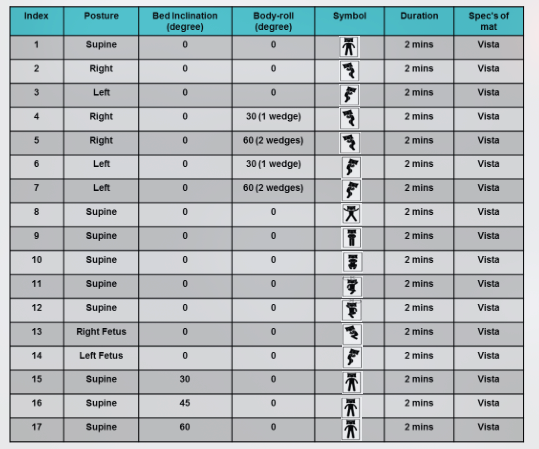
\includegraphics[width=0.5\linewidth]{position_tables.png}
    \caption{Tabla de posiciones de las personas en el experimento I}
    \label{fig:experimento_I}
\end{figure}
Para el experimento 1, cada paciente 17 archivos de texto que contienen en cada línea la imagen de $64 \times 32$ flattenizada, dando un fila con 2048 columnas. Cada archivo contiene tamaños diferentes de tomas o muestras.

Para el experimento 2, se tomaron más posiciones de cada lado, sin embargo se hizo con dos tipos de camas diferentes. de aire y de esponja. Cada cama tiene un tamaño de queen size,\cite{baran2017pressure} . Para el caso de las imágenes tomadas en el experimento 2, cada paciente tiene su carpeta de imágenes con las que tiene los dos tipos de camas y en el nombre se adjunta el nombre de la posición tomada (Figura \ref{fig:Experimento2})

\begin{figure}[h!]
\centering

\begin{subfigure}{0.3\textwidth}
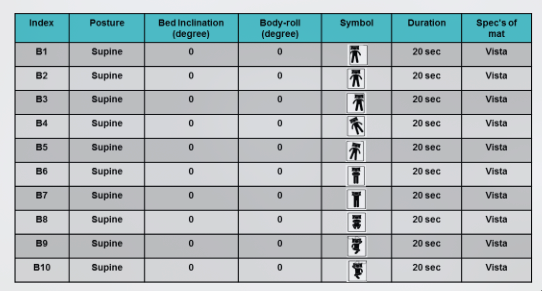
\includegraphics[width=\linewidth]{partb.png}
\caption{1}
\end{subfigure}
\begin{subfigure}{0.3\textwidth}
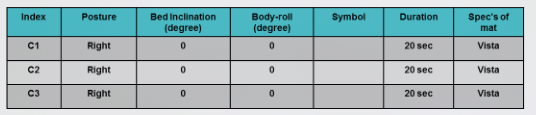
\includegraphics[width=\linewidth]{partc.png}
\caption{2}
\end{subfigure}
\begin{subfigure}{0.3\textwidth}
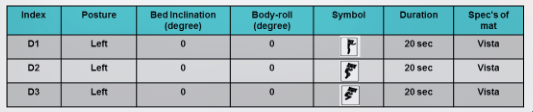
\includegraphics[width=\linewidth]{partd.png}
\caption{3}
\end{subfigure}

\begin{subfigure}{0.3\textwidth}
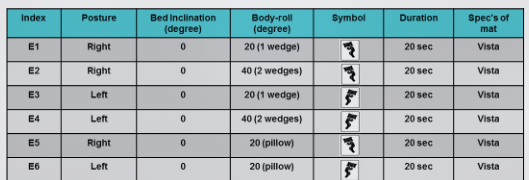
\includegraphics[width=\linewidth]{parte.png}
\caption{4}
\end{subfigure}
\begin{subfigure}{0.3\textwidth}
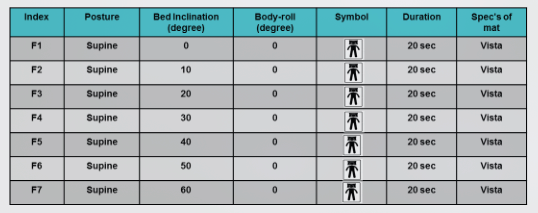
\includegraphics[width=\linewidth]{partf.png}
\caption{5}
\end{subfigure}
\caption{Conjunto de tablas de las figuras con sus respectivas posiciones del experimento 2}
\label{fig:Experimento2}
\end{figure}

\section {separación de los conjuntos de datos}
Para ello se debió de implementar un script en python que permita la lectura de las carpetas y la lectura de los archivos. Con el experimento 1, la organización de las carpetas es más sencillo, ay que en al raíz de esa carpeta, contiene las carpetas de los pacientes y dentro contiene las imágenes.
Para facilitar la clasificación, ya que fueron varias posiciones tomadas por paciente, y en cada posición no tienen la misma cantidad de información, y para no convertir el problema de con demasiadas clases, se decide utilizar solamente 3 clases, posiciones que estén a la izquierda, a la derecha y al centro.
Al separar cada posición acorde a lo que se ve en (Figura \ref{fig:experimento_I}) , se calculan las muestras por clase y hay menos muestras para el lado izquierdo y para el lado derecho. por lo que el proceso siguiente fue hacer una aumentación de datos. Con la aumentación de los datos, cada clase tendría 10314 muestras.
Para el caso del experimento 2, primero se separo por tipo de cama, y el proceso de la toma de muestra fue similar, sin embargo, la diferencias que en el archivo de texto, la matriz de la imagen de presión ya no se encontraba flattenizado, sino que cada columna y renglón corresponde al tamaño original de la imagen, siendo las imágenes de $64 \times 27$
\section{Aumentación de los datos}
Se utilizaron pocos filtros y que dieran poca variación al conjunto de la imágenes originales, ya que la diferencia entre el label de las imágenes de la derecha y de la izquierda era de 6000 imágenes, por lo que las imágenes que se necesitaban tenían que ser de menor variación posible. Rotación de imágenes con un ángulo máximo de 10 grados positivo y negativo y ruido gaussiano, con un valor de media en 0 y de desviación de $0.02$.
Estos filtros también se le aplicaron al segundo experimento. 
Al haberse aumentado, el conjunto de datos del experimento 1, llego a tener una longitud de 31839 muestras, por lo tanto, para cada categoría habrían 10613 muestras.
Para el caso del experimento 2, se decidió usar los diferentes tipos de cama por separado. En cada tipo de cama hay 1260 muestras, originalmente tenía menos, y al hacer el split de $70/30$, se des-balanceaba, así que se necesito balancear a 420 muestras por categoría.
\section{Calculo de características}
El método utilizado para calcular las características fue el HoG, o Histograma de gradientes orientados, que en resumen, el método intenta preservar las características de bordes y texturas de una imagen.
A los dos experimentos se les implementó el método mencionado, sin antes haber normalizado la imagen. Esta función retorna un vector de características. Se vuelve a calcular un vector de características HoG con 9 orientaciones para adquirir 41 elementos del vector nuevo para que sean parte de las características 
\begin{itemize}
    \item Media
    \item Desviación estándar
    \item Máximo
    \item Mediana
    \item Cuartil 1 
    \item Cuartil 3
    \item Sesgo
    \item Kurtosis
    \item Energía 
\end{itemize}
Se guardan ambos los cálculos de los experimentos en CSV. Para el caso del experimento 2, se hacen 2 CSV, uno para el esponja y otro para el de aire.
\section{Modelos}
Los modelos que se entrenaron fueron 
\begin{itemize}
    \item KNN
    \begin{itemize}
        \item Fine
        \item Medium
        \item Coarse
        \item Weighted
        \item Minkowski
        \item Cosine
    \end{itemize}

    \item SVM
    \begin{itemize}
        \item Lineal
        \item Cuadrático
        \item Cúbico
        \item Quinto
        \item RBF
    \end{itemize}

    \item Árboles
    \begin{itemize}
        \item Decision Tree
        \item Random Forest
        \item AdaBoost
        \item GradientBoost
    \end{itemize}

    \item Bayesiano
    \begin{itemize}
        \item Gaussiano
        \item Kernel
    \end{itemize}

    \item LDA
\end{itemize}
A cada modelo se le sacó su curva de aprendizaje, matriz de confusión y una curva ROC 
\chapter{Resultados}
Muchos de los modelos terminaron con sobreeentrenamientos significativos,algunos ni siquiera del sobre entrenamiento inicial lograron recuperarse para converger juntos


El proceso se puede resumir en el diagrama de la figura \ref{fig:diagrama}
\begin{figure}[h!]
\centering

\begin{tikzpicture}[
    node distance=1.5cm and 2.5cm,
    >=latex,
    process/.style={rectangle, rounded corners, draw, align=center, minimum width=4.2cm, minimum height=1cm},
    model/.style={rectangle, draw, align=left, minimum width=4cm, minimum height=1cm},
    group/.style={rectangle, rounded corners, draw, dashed, inner sep=0.35cm}
]

% NODES (Pipeline)
\node[process] (read) {Lectura de datos};
\node[process, below=of read] (labeling) {Labeling correcto y \\ ordenamiento de imágenes};
\node[process, below=of labeling] (aug) {Aumentación de datos};
\node[process, below=of aug] (hog) {Cálculo de características HoG \\ y estadísticas};
\node[process, below=of hog] (save) {Guardar 3 conjuntos de datos};
\node[process, below=of save] (scale) {Escalar y aplicar PCA};
\node[process, below=of scale] (train) {Entrenamiento con varios modelos};
\node[process, below=of train] (plot) {Graficar y mostrar resultados};

% MODEL GROUPS
\node[group, right=4.5cm of train, align=left] (models) {
    \begin{minipage}{5.2cm}
    \textbf{Modelos de Machine Learning}
    \vspace{0.2cm}

    \textbf{KNN}\\
    - Fine\\
    - Medium\\
    - Coarse\\
    - Weighted\\
    - Minkowski\\
    - Cosine\\[3pt]

    \textbf{SVM}\\
    - Lineal\\
    - Cuadrático\\
    - Cúbico\\
    - Quinto grado\\
    - RBF\\[3pt]

    \textbf{Árboles}\\
    - Decision Tree\\
    - Random Forest\\
    - AdaBoost\\
    - GradientBoost\\[3pt]

    \textbf{Bayesiano}\\
    - Gaussiano\\
    - Kernel\\[3pt]

    \textbf{LDA}
    \end{minipage}
};

% ARROWS (Pipeline)
\draw[->] (read) -- (labeling);
\draw[->] (labeling) -- (aug);
\draw[->] (aug) -- (hog);
\draw[->] (hog) -- (save);
\draw[->] (save) -- (scale);
\draw[->] (scale) -- (train);
\draw[->] (train) -- (plot);

% Arrow from pipeline to model list
\draw[->] (train.east) -- (models.west);

\end{tikzpicture}

\caption{Diagrama del flujo completo del proceso de Machine Learning.}
\label{fig:diagrama}
\end{figure}


\begin{table}[h!]
    \resizebox{0.8\textwidth}{!}{%
    \begin{tabular}{lcccccc}
    \toprule
    \textbf{Modelo} & \textbf{Accuracy} & \textbf{Precision} & \textbf{Recall} & \textbf{F1 Score} & \textbf{auc macro} & \textbf{auc micro} \\
    \midrule
    KNN Coarse & 97.66 & 97.69 & 97.66 & 97.65 & 99.87& 99.85\\
    KNN Cosine & 98.31 & 98.33 & 98.31 & 98.31 & 99.99 & 99.89 \\
    KNN Fine & 98.63 & 98.63 & 98.63 & 98.63 & 99.69 & 99.69 \\
    KNN Medium & 98.59 & 98.60 & 98.59 & 98.59 & 99.82& 99.82\\
    KNN Minkowski & 98.23 & 98.24 & 98.23 & 98.22 & 99.88 & 99.87 \\
    KNN Weighted & 98.46 & 98.47 & 98.46 & 98.45  & 99.89 & 99.89\\
    SVM Lineal & 92.16 & 92.15 & 92.16 & 92.13 & 98.34&98.34 \\
    SVM Quadratic & 97.20 & 97.20 & 97.20 & 97.20 & 966&99.66 \\
    SVM Qubic & 98.93 & 98.93 & 98.93 & 98.93 & 99.91 & 99.91 \\
    SVM RBF & 97.67 & 97.68 & 97.67 & 97.67 & 99.84& 99.85\\
    SVM Fifth & 96.81 & 96.99 & 96.81 & 96.82 & 99.84 & 99.83 \\
    Gaussian & 89.96 & 88.98 & 88.95 & 88.89 & 96.97 &97.08 \\ 
    Kernel Bayes & 98.69 & 98.69 & 98.69 & 98.69 & 99.97 & 99.96 \\
    Decision & 86.58 & 86.58 & 86.58 & 86.58 & 96.23 & 96.27 \\
    RF & 95.69 & 95.70 & 95.69 & 95.69 & 99.67 & 99.66 \\
    Ada & 85.48 & 85.47 & 85.48 & 85.40 & 94.99 & 95.17 \\ 
    Gradient & 96.98 & 96.98 & 96.98 & 96.98 & 99.76 & 99.76 \\
    LDA  & 91.64& 91.62 & 91.64 & 91.60 & 98.62 & 98.67 \\
    \bottomrule
    \end{tabular}}
    \caption{Experimento 1}
    \label{tab:experimento1}
\end{table}
Si bien, los resultados que observamos de los Knn para el experimento 1, vistos en la tabla \ref{tab:experimento1}. Todos los modelos de Knn se sobre ajustan, y el que mejor da, sin sobre ajustarse demasiado es el Minkowski con un accuracy de 98.23 (fig \ref{fig:E1Knn}).
Para los modelos de support vector machine. Tienen la particularidad de saber al principio mucho, sin embargo, para este caso, ningún modelo en un principio llega con el temible 1.0 de accuracy en el train, sino como en el 99.5 de accuracy. Conforme va avanzando el entrenamiento, se van ajustando y buscan un punto de convergencia. EL que mejor resultado da es el RBF con 97.67 (fig \ref{fig:E1SVM}).
Este modelo se escogió usan PCA con 95 de varianza. Muchos modelos siguientes, el PCA les apoyo en mejorar sus curvas de aprendizaje
Por la parte de los bayesianos. El Bayesiano con kernel gaussiano fue el que mejor dio, teniendo su comportamiento clásico de sobre ajuste inicial, y ajustarse hasta encontrar un punto de convergencia entre el entrenamiento y la validación (fig \ref{fig:E1Naive}). Pero este modelo se obtuvo al aplicarle un PCA del 95 de varianza, ya que con la forma natural del conjunto, tendía al sobre ajuste.
Por la parte de los árboles, todos los árboles en todos los experimentos mejoraron al aplicarles una reducción de dimensionalidad por medio del PCA. El Gradient Boost mejoro sustancialmente, ya que la curva de entrenamiento sin PCA, siempre se mantenía en 100, mientras que con el PCA, su curva empezó en 99.5 y bajo a converger junto el valor de validación (fig \ref{fig:E1GRad}).. Aunque otro buen candidato es el Decision tree que obtuvo una mejor muestra de convergencia a diferencia del Random Forest. En este experimento, cuando se entrenó el LDA sin reducción de dimensionalidad, se sobre ajustaba con la curva de entrenamiento de 1, sin embargo, al haberse aplicado un PCA, la curva mejoró, en la validación, luego saltaba a valores mayores que entrenamiento.
Esto se puede observar en las siguientes gráficas.


\begin{figure}[h!]
\centering

\begin{subfigure}{0.3\textwidth}
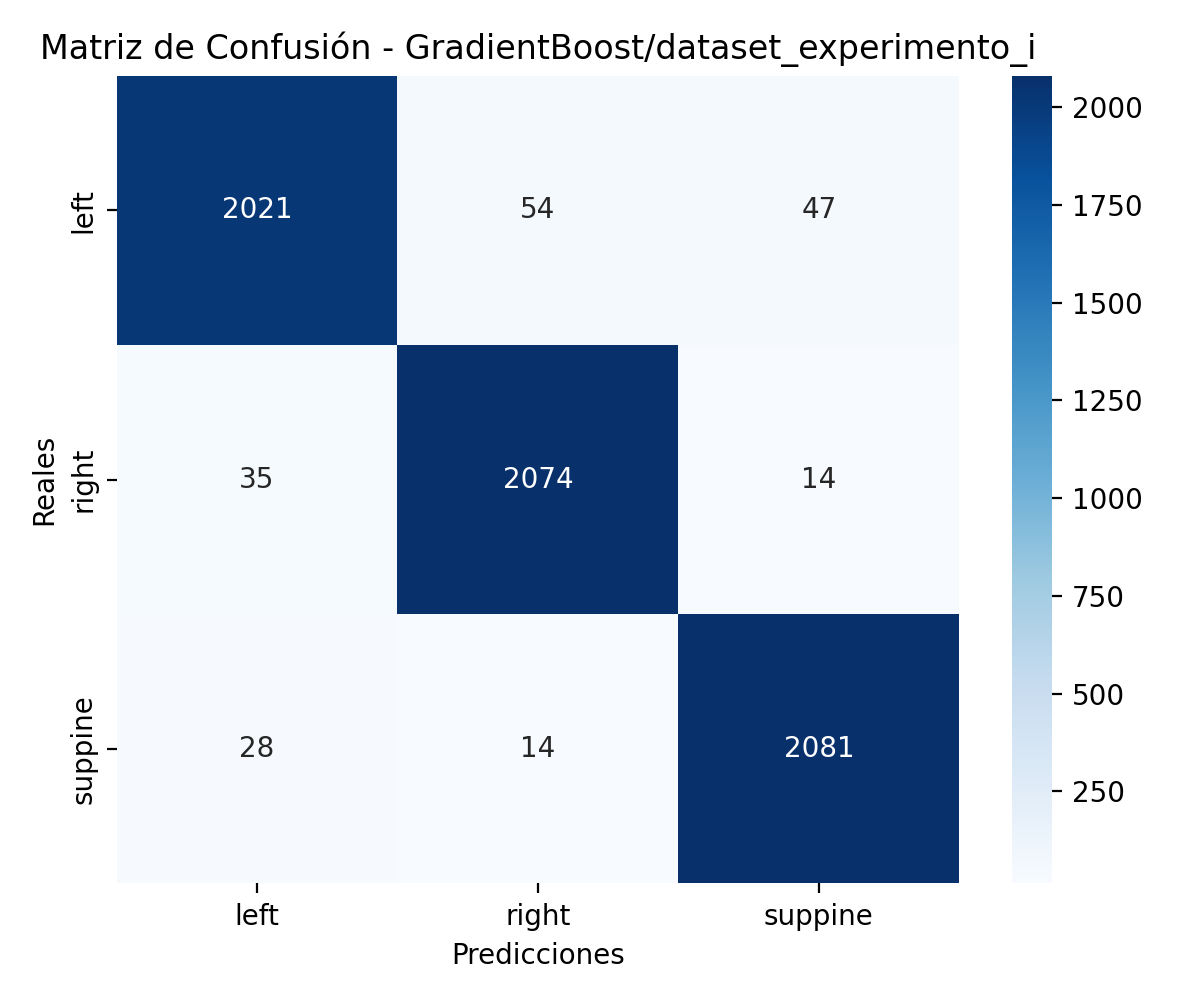
\includegraphics[width=\linewidth]{experimento1/arbol/dataset_experimento_i_confusion_matrix.png}
\caption{1}
\end{subfigure}
\begin{subfigure}{0.3\textwidth}
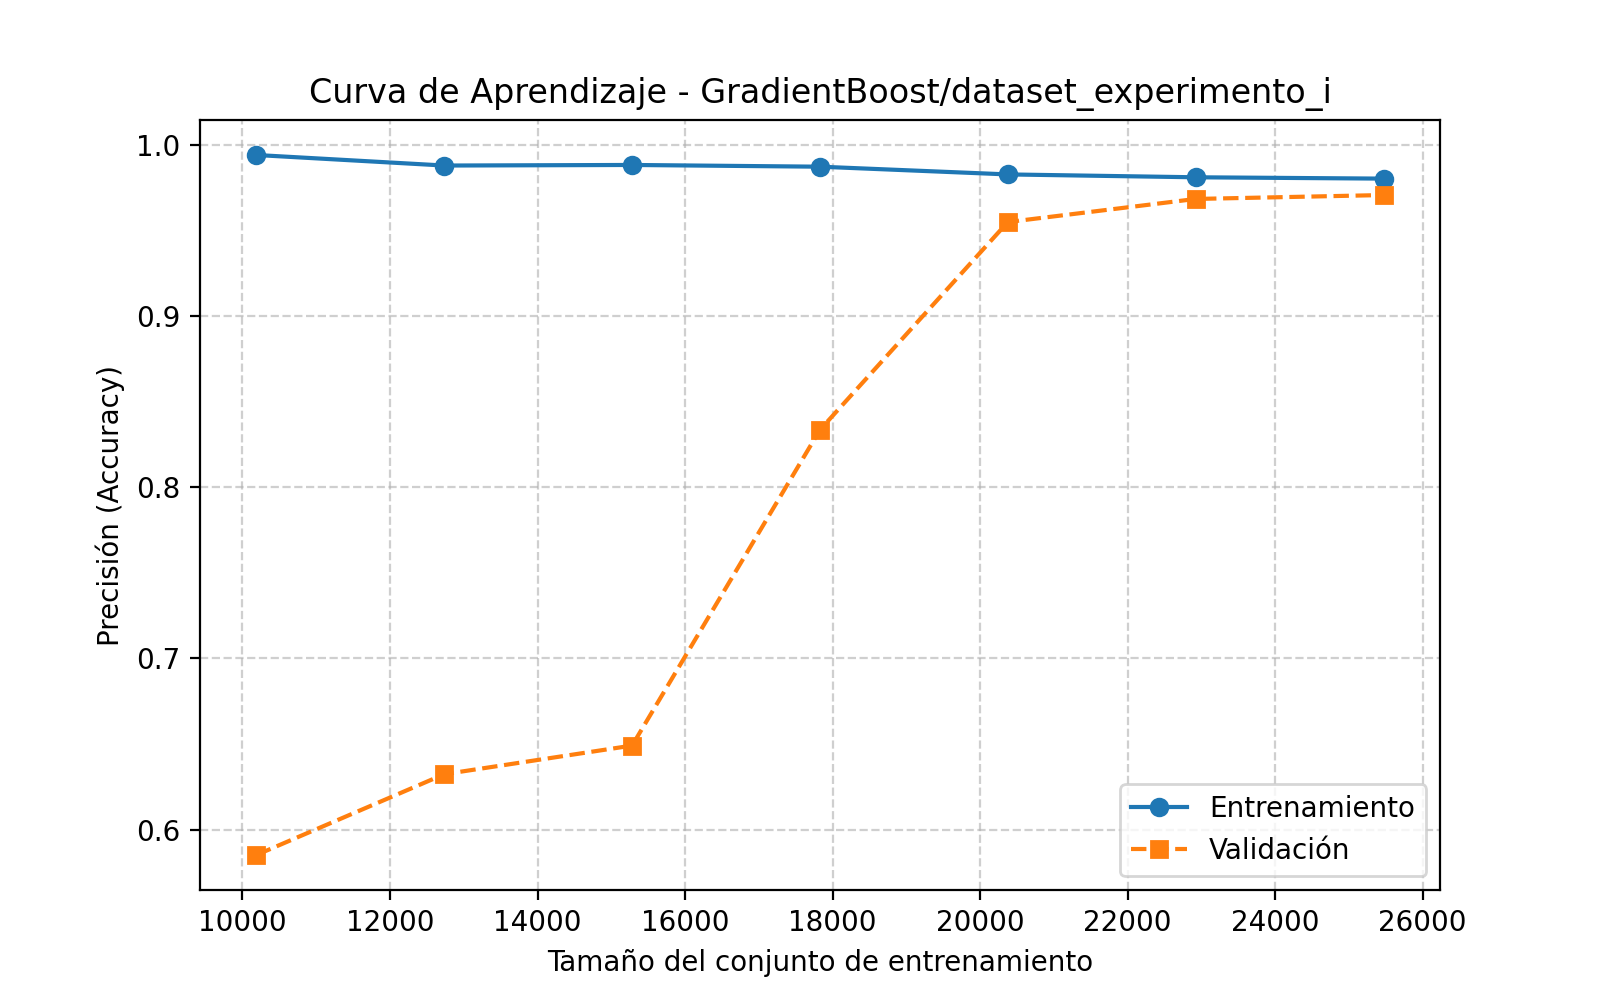
\includegraphics[width=\linewidth]{experimento1/arbol/dataset_experimento_i_learning_curve.png}
\caption{2}
\end{subfigure}
\begin{subfigure}{0.3\textwidth}
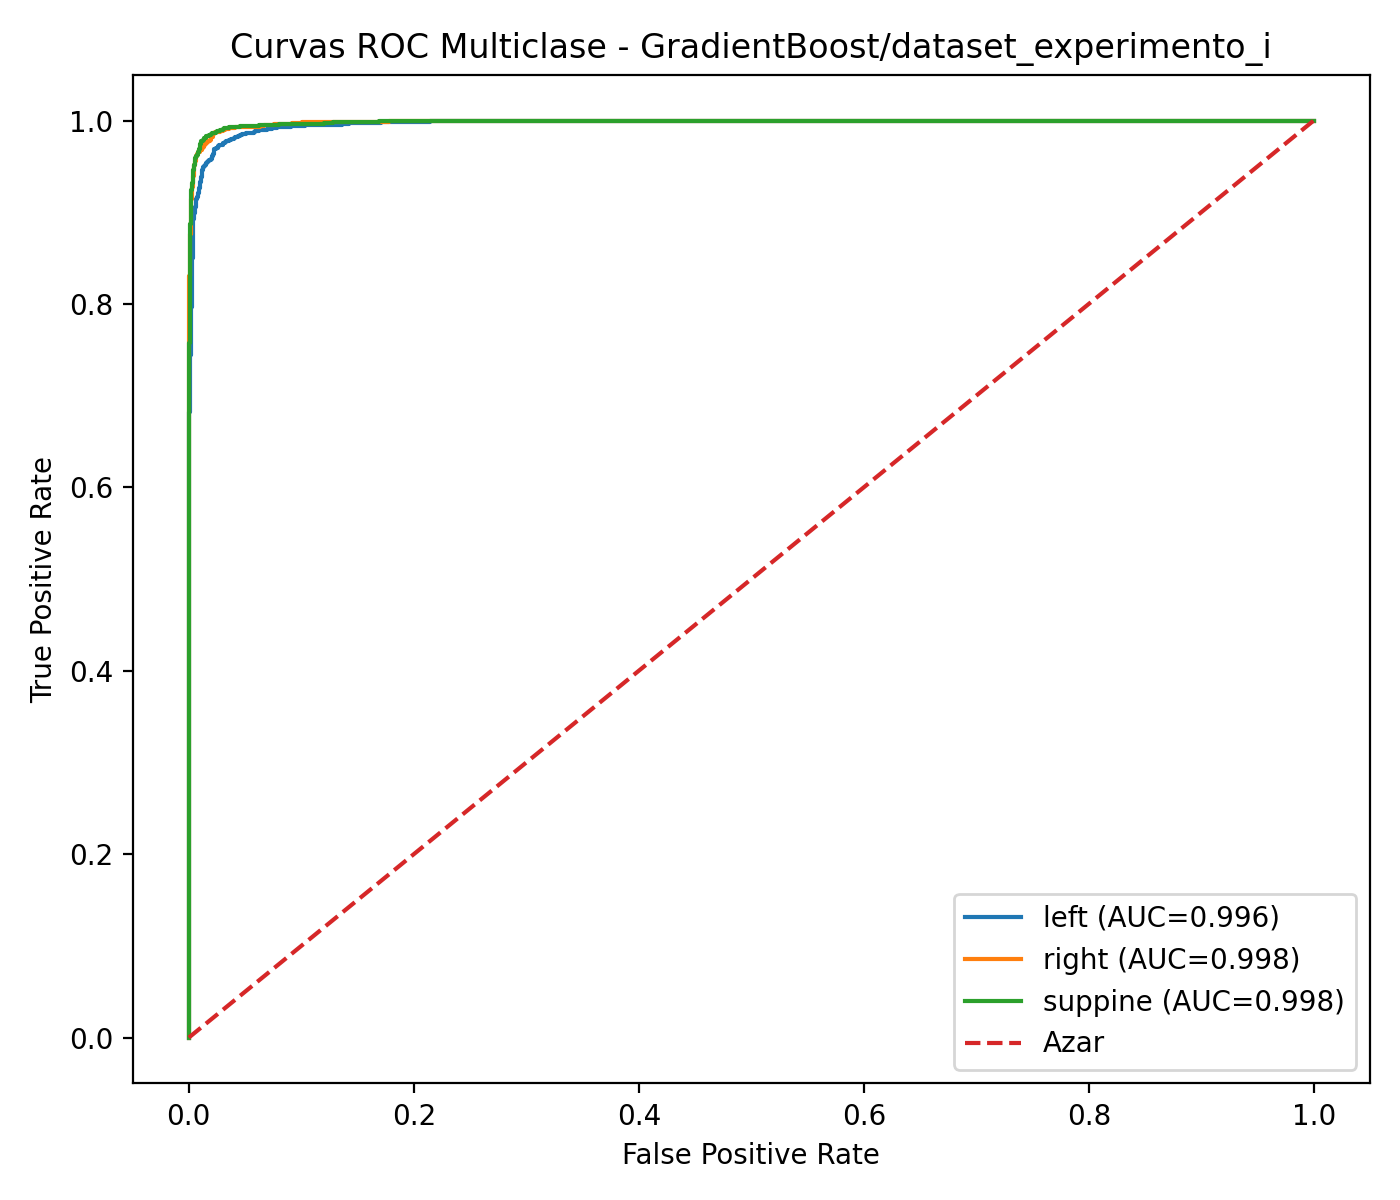
\includegraphics[width=\linewidth]{experimento1/arbol/dataset_experimento_i_multiclass_roc.png}
\caption{3}
\end{subfigure}
\caption{La matriz de confusión, la curva de aprendizaje y la curva ROC para el GradientBoost}
\label{fig:E1GRad}
\end{figure}


\begin{figure}[h!]
\centering

\begin{subfigure}{0.3\textwidth}
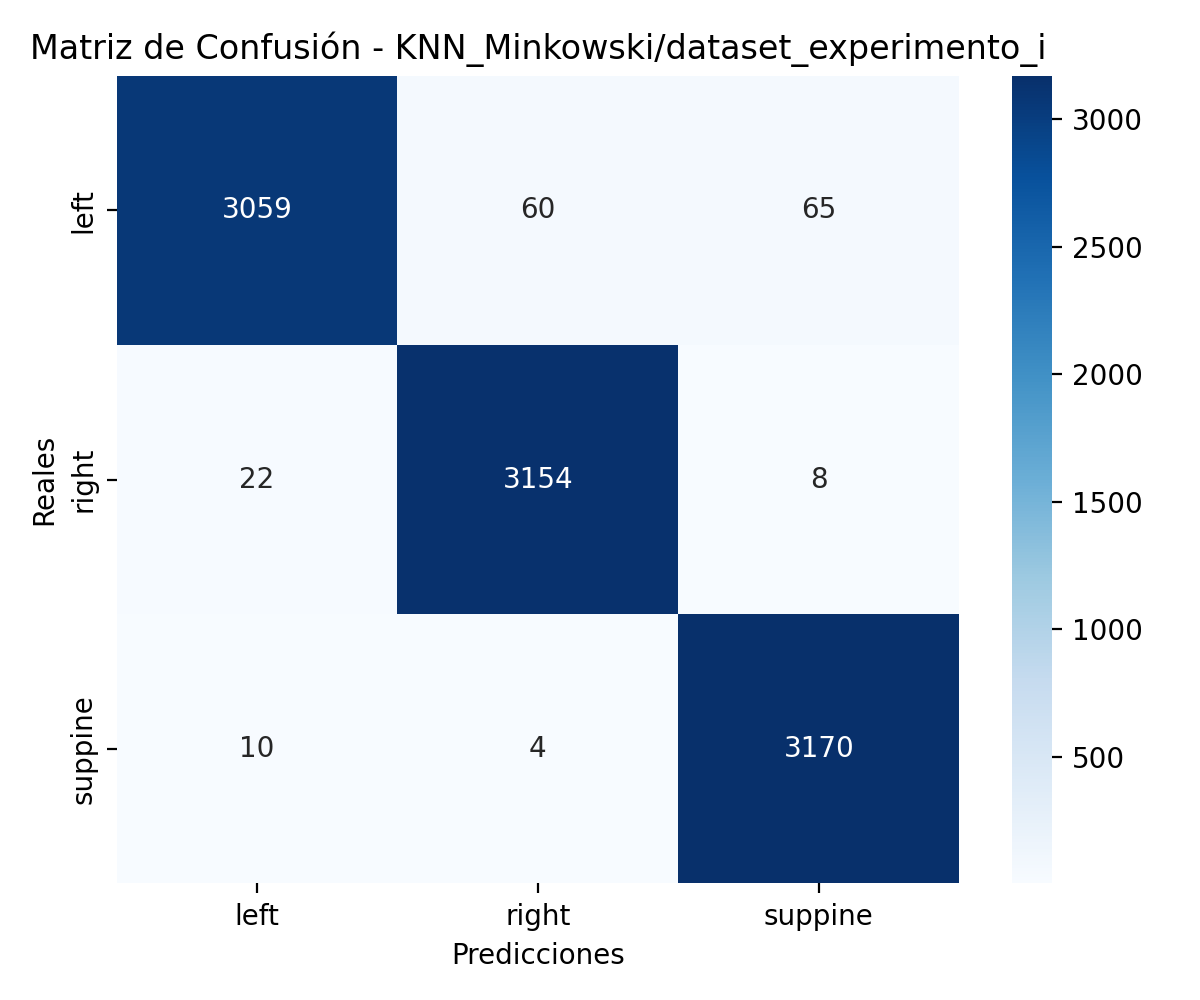
\includegraphics[width=\linewidth]{experimento1/knn/dataset_experimento_i_confusion_matrix.png}
\caption{1}
\end{subfigure}
\begin{subfigure}{0.3\textwidth}
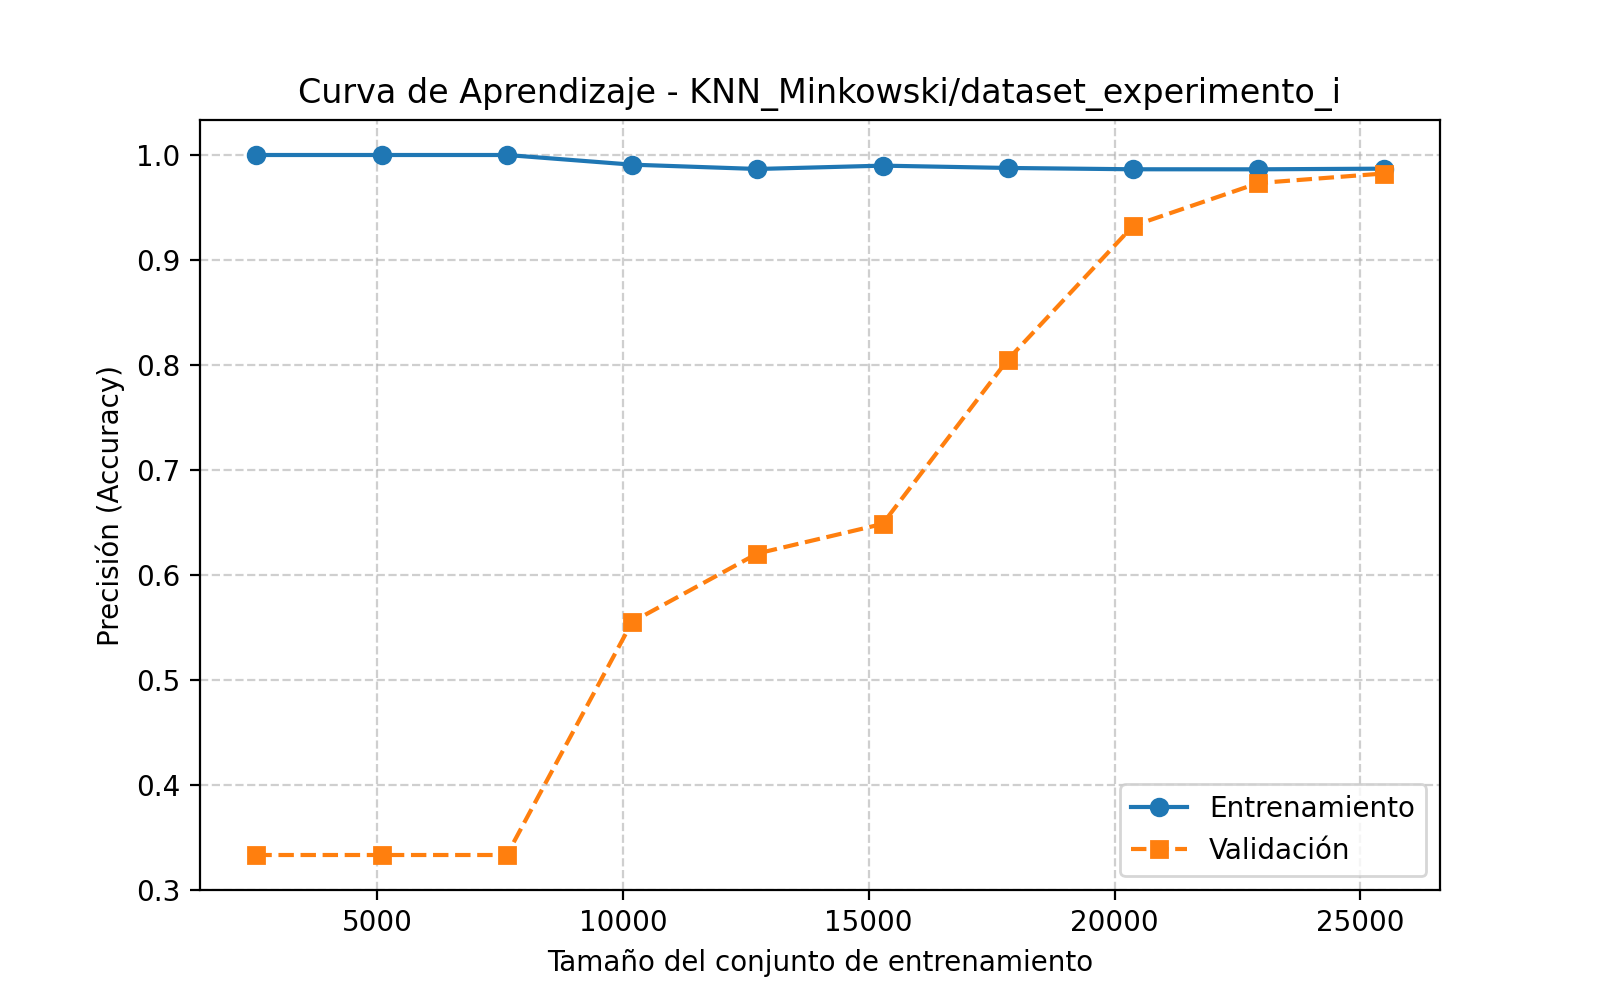
\includegraphics[width=\linewidth]{experimento1/knn/dataset_experimento_i_learning_curve.png}
\caption{2}
\end{subfigure}
\begin{subfigure}{0.3\textwidth}
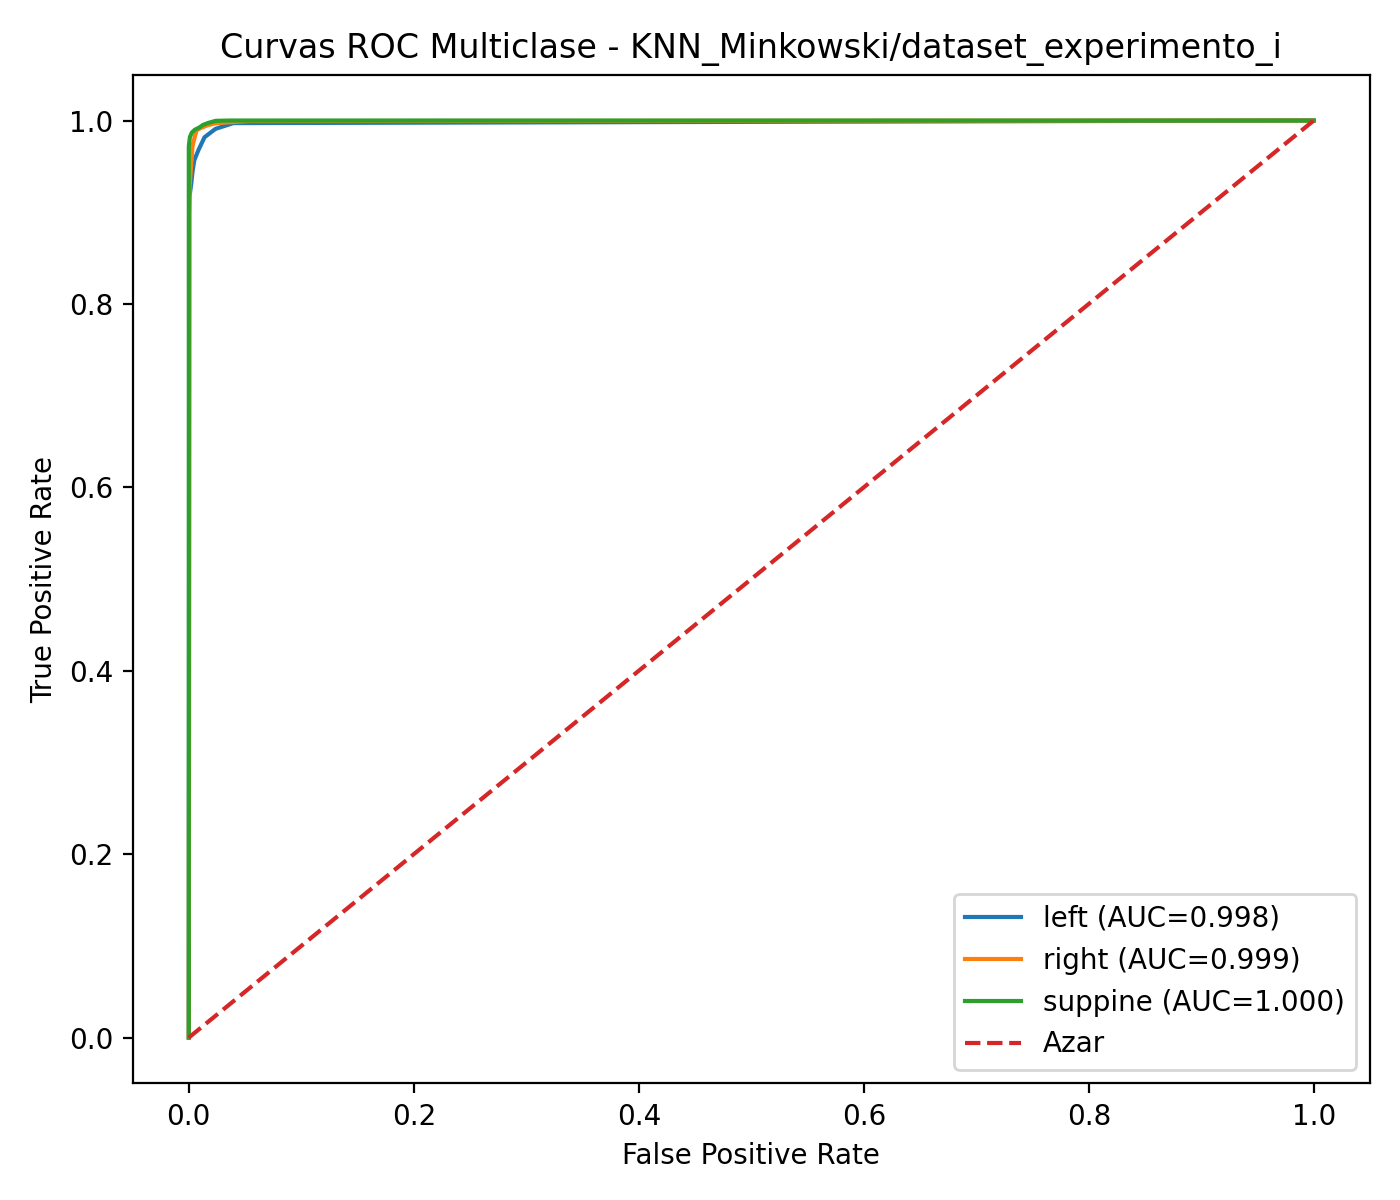
\includegraphics[width=\linewidth]{experimento1/knn/dataset_experimento_i_multiclass_roc.png}
\caption{3}
\end{subfigure}
\caption{La matriz de confusión, la curva de aprendizaje y la curva ROC para el Knn}
\label{fig:E1Knn}
\end{figure}


\begin{figure}[h!]
\centering

\begin{subfigure}{0.3\textwidth}
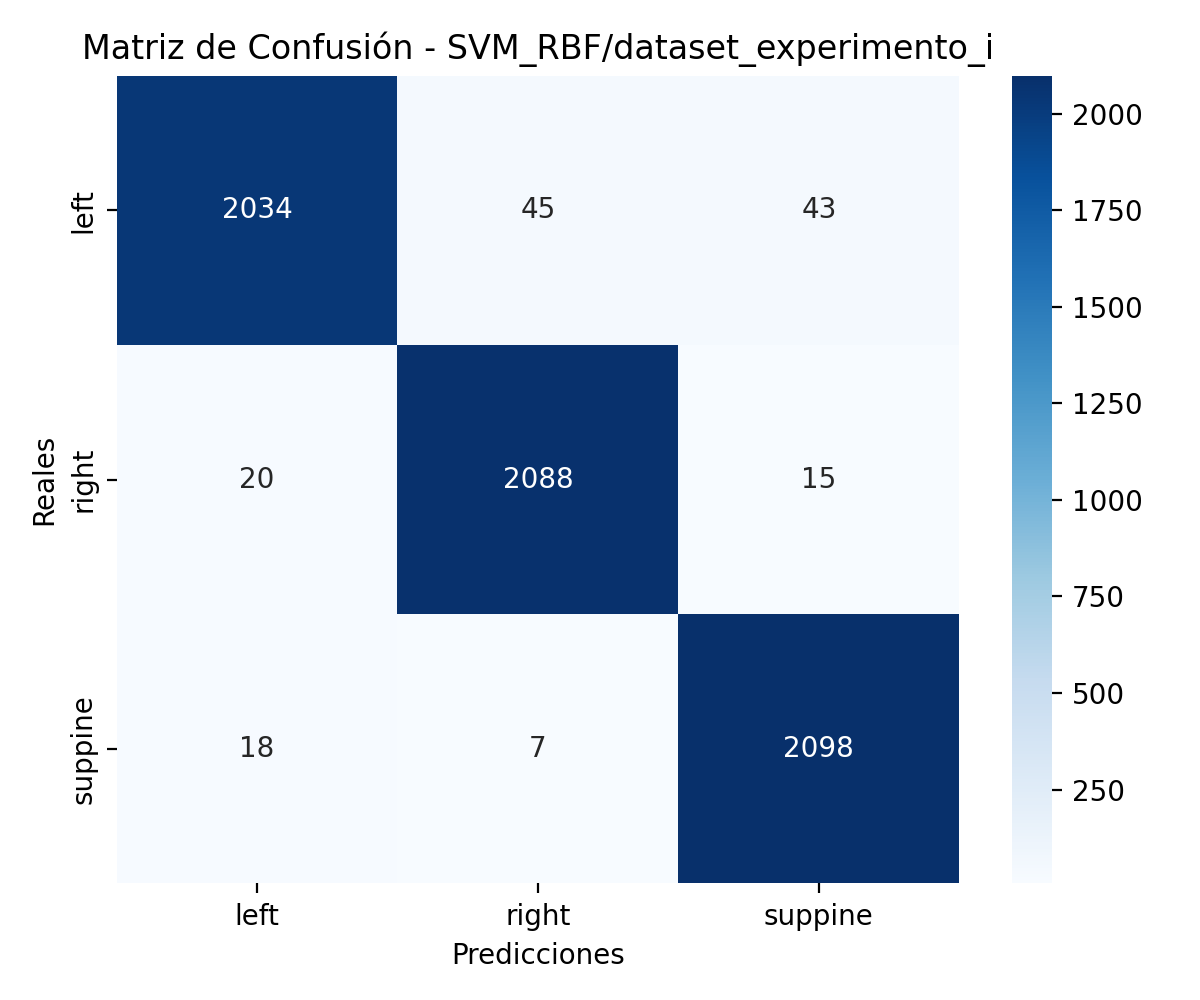
\includegraphics[width=\linewidth]{experimento1/svm/dataset_experimento_i_confusion_matrix.png}
\caption{1}
\end{subfigure}
\begin{subfigure}{0.3\textwidth}
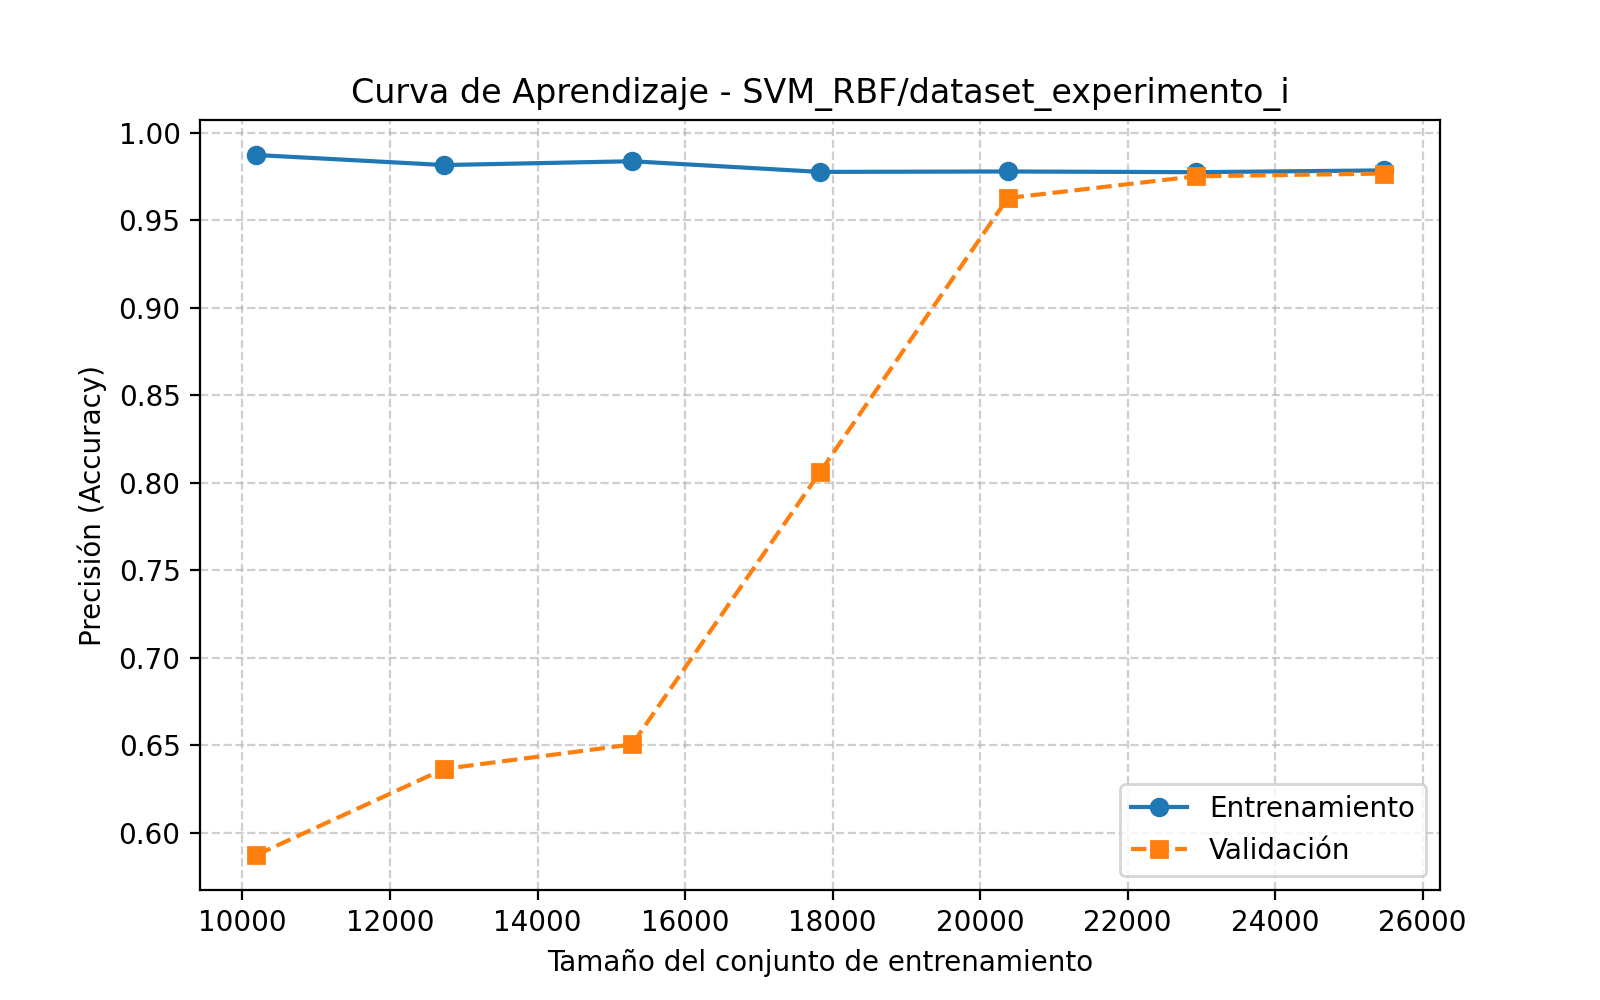
\includegraphics[width=\linewidth]{experimento1/svm/dataset_experimento_i_learning_curve.png}
\caption{2}
\end{subfigure}
\begin{subfigure}{0.3\textwidth}
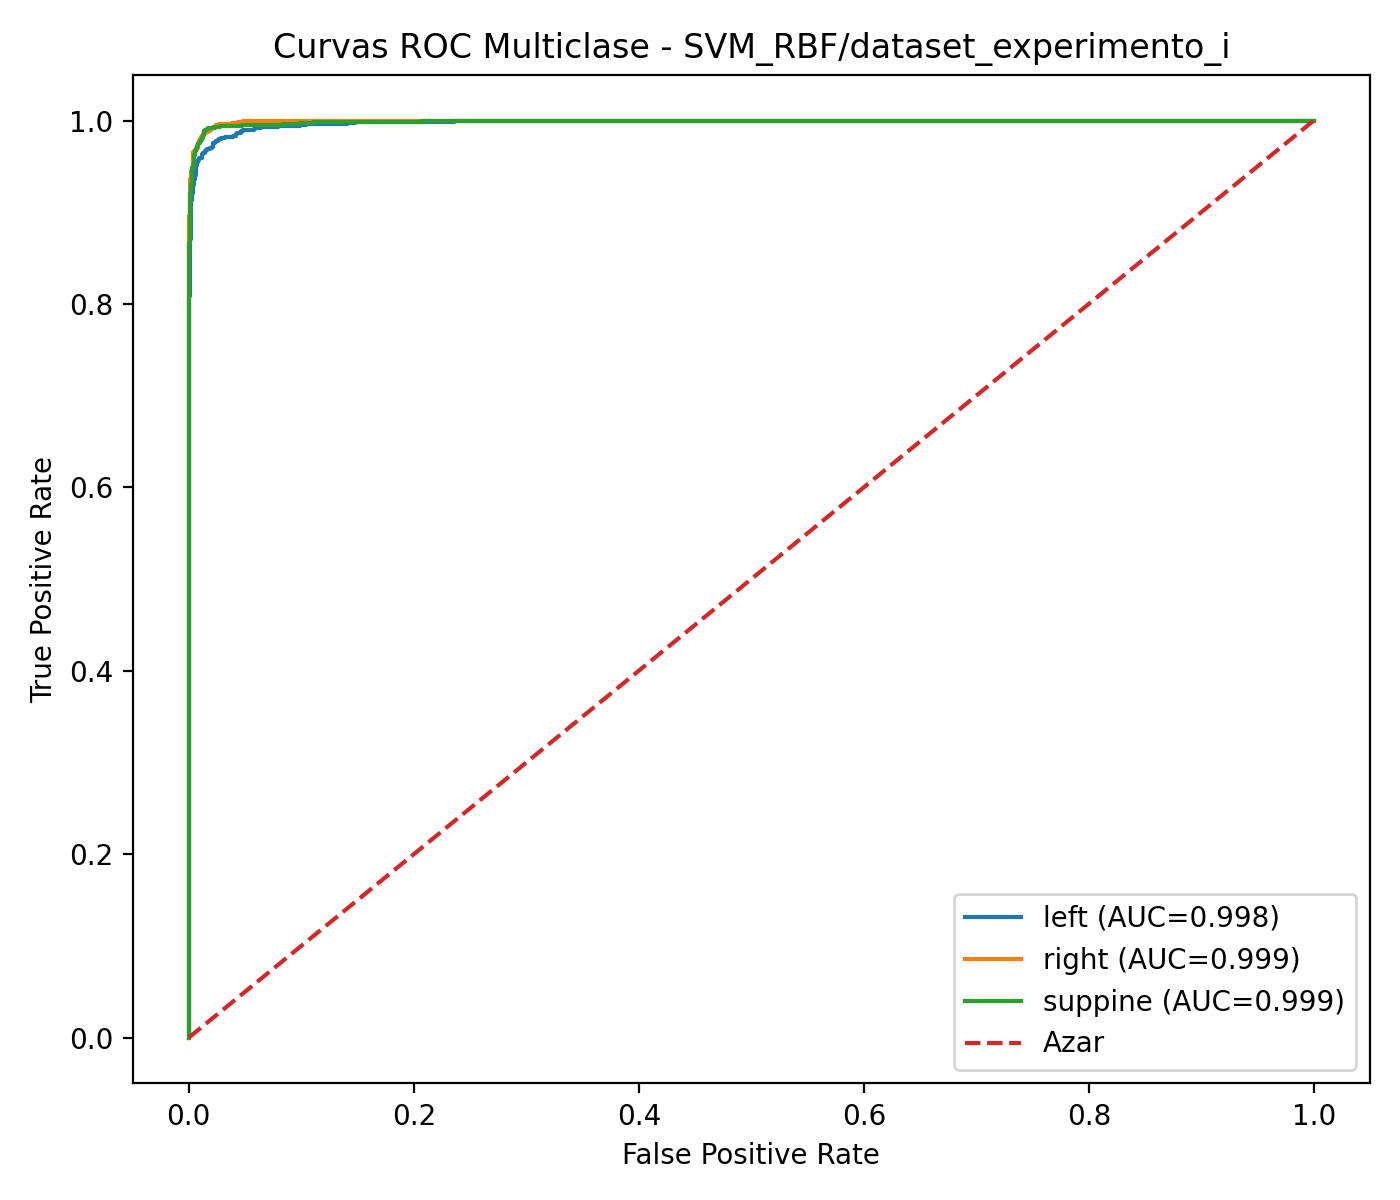
\includegraphics[width=\linewidth]{experimento1/svm/dataset_experimento_i_multiclass_roc.png}
\caption{3}
\end{subfigure}
\caption{La matriz de confusión, la curva de aprendizaje y la curva ROC para el Support Vector Machine}
\label{fig:E1SVM}
\end{figure}


\begin{figure}[h!]
\centering

\begin{subfigure}{0.3\textwidth}
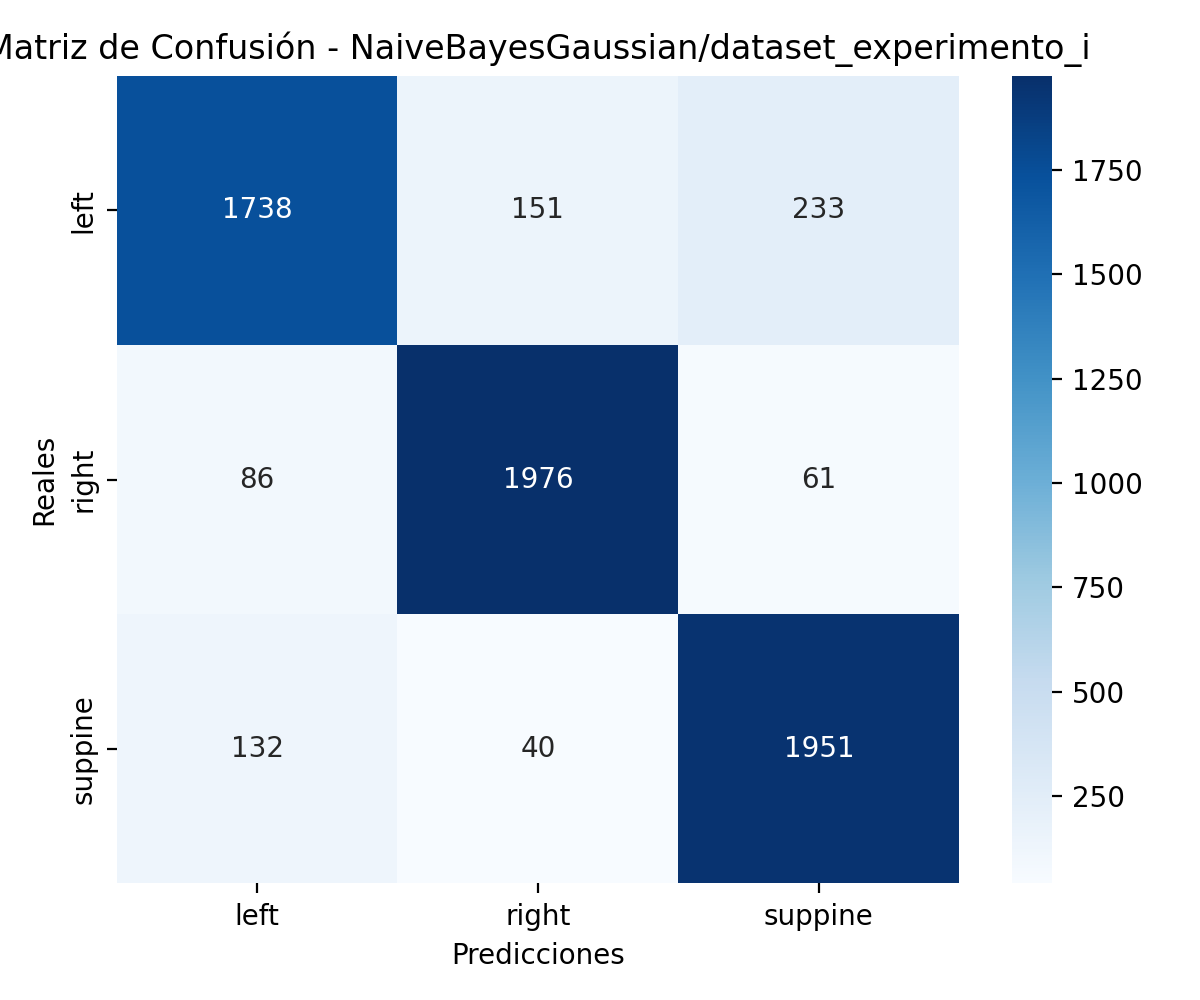
\includegraphics[width=\linewidth]{experimento1/bayesiano/dataset_experimento_i_confusion_matrix.png}
\caption{1}
\end{subfigure}
\begin{subfigure}{0.3\textwidth}
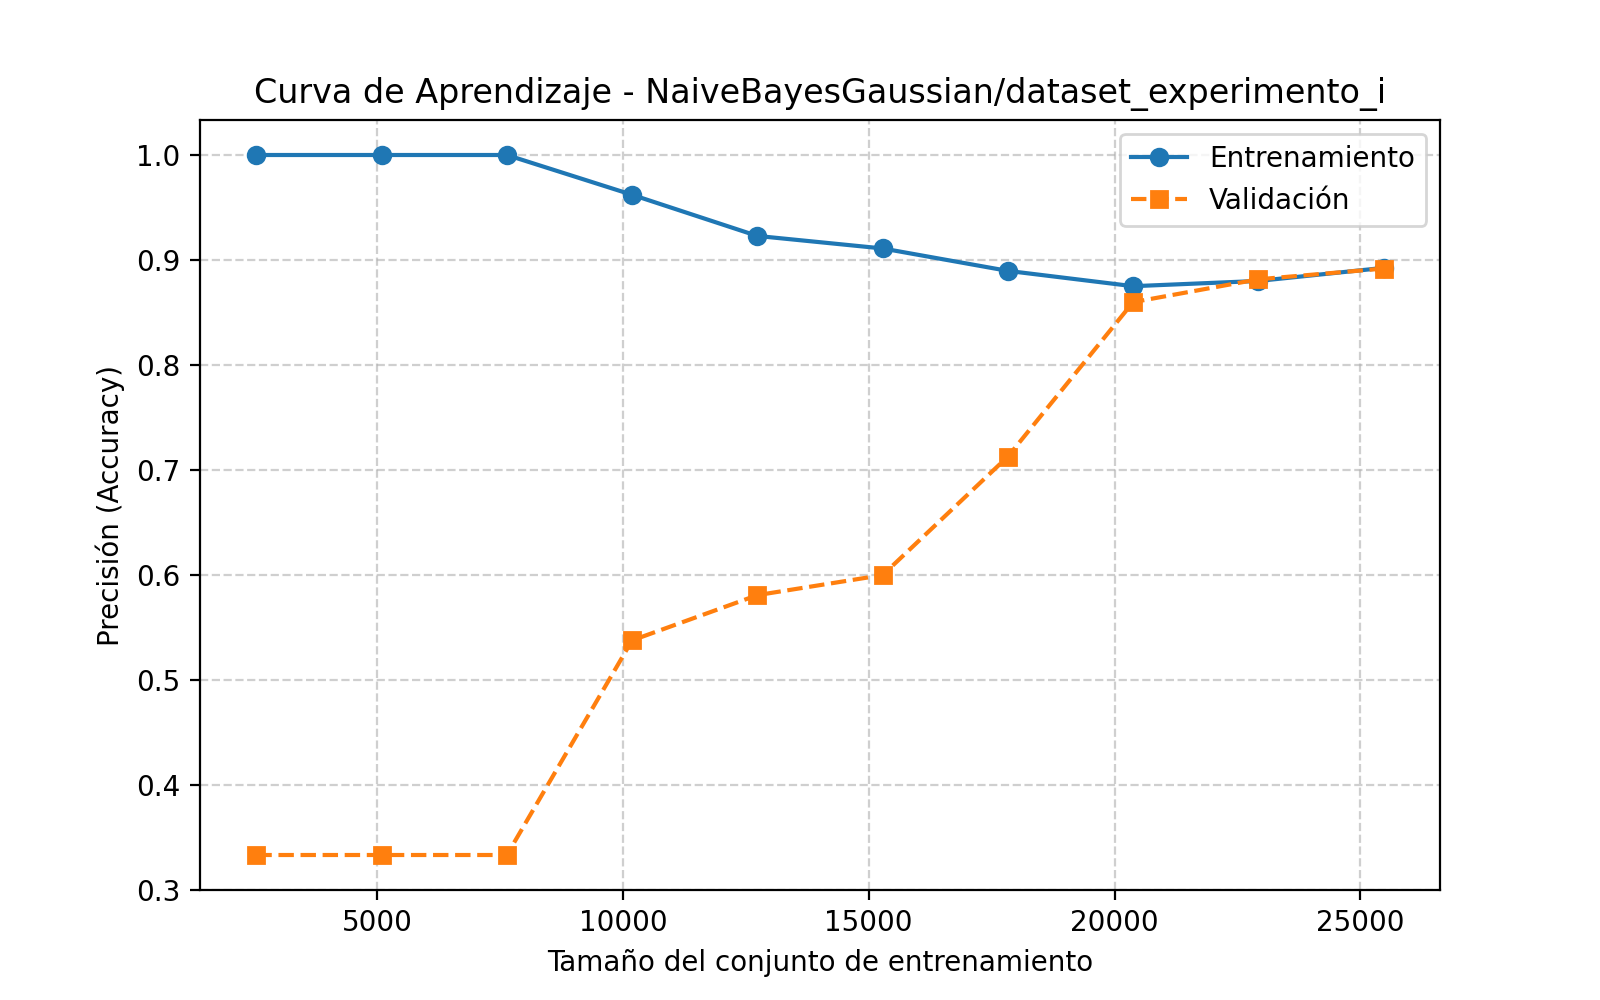
\includegraphics[width=\linewidth]{experimento1/bayesiano/dataset_experimento_i_learning_curve.png}
\caption{2}
\end{subfigure}
\begin{subfigure}{0.3\textwidth}
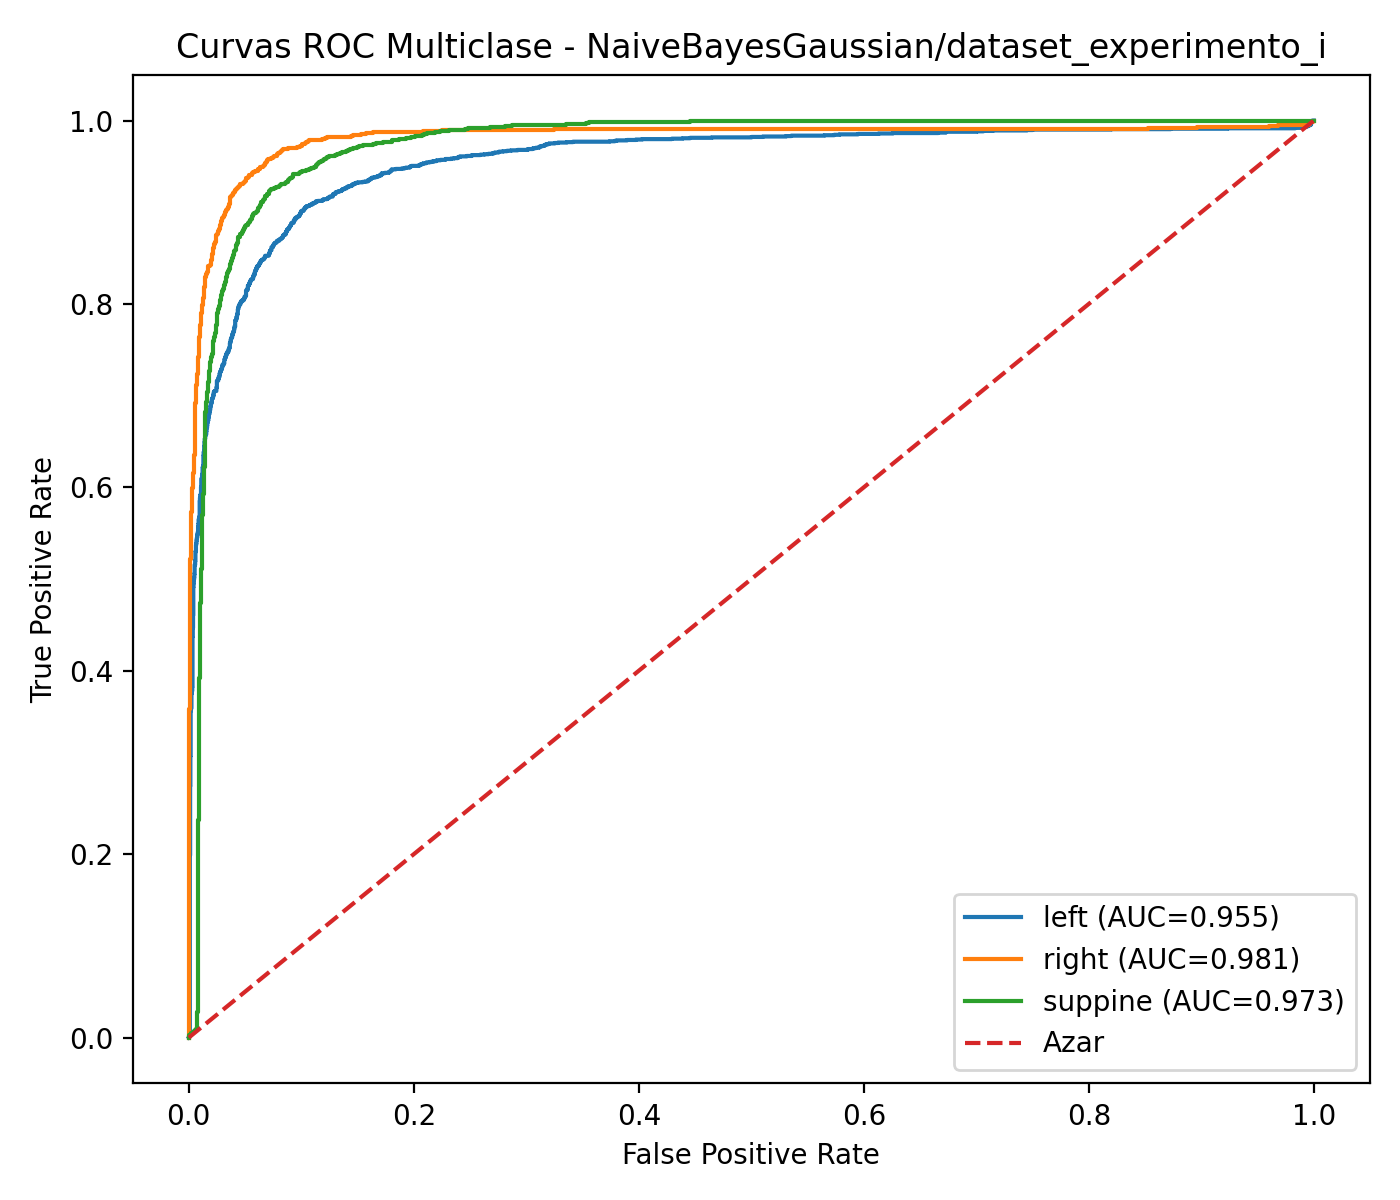
\includegraphics[width=\linewidth]{experimento1/bayesiano/dataset_experimento_i_multiclass_roc.png}
\caption{3}
\end{subfigure}
\caption{La matriz de confusión, la curva de aprendizaje y la curva ROC para el Naive Bayes}
\label{fig:E1Naive}
\end{figure}


    \begin{table}[h!]
    \resizebox{0.8\textwidth}{!}{%
    \begin{tabular}{lcccccc}
    \toprule
    \textbf{Modelo} & \textbf{Accuracy} & \textbf{Precision} & \textbf{Recall} & \textbf{F1 Score} & \textbf{auc macro} & \textbf{auc micro} \\
    \midrule
    KNN Coarse & 75.39 & 76.71 & 75.39 & 75.71 & 87.81& 88.01\\
    KNN Cosine & 75.92 & 78.03 & 75.92 & 76.24 & 92.40 & 92.36 \\
    KNN Fine & 83.59 & 84.15 & 83.59 & 83.72 & 93.36 & 93.35 \\
    KNN Medium & 79.36 & 79.98 & 79.36 & 79.54 & 91.98 & 92.05 \\
    KNN Minkowski & 75.13 & 76.73 & 75.13 & 75.43 & 89.52 & 89.65 \\
    KNN Weighted & 83.34 & 83.55 & 83.39 & 83.39  & 94.24 & 94.32\\
    SVM Lineal & 94.97 & 95.16 & 94.97 & 94.91 & 98.98 & 99.27 \\
    SVM Quadratic & 98.94 & 98.95 & 98.94 & 98.94 & 1.0&99.99 \\
    SVM Qubic & 98.14 & 98.20 & 98.14 & 98.14 & 99.99 & 99.99 \\
    SVM RBF & 99.47 & 99.47 & 99.47 & 99.47 & 1.0 & 99.99 \\
    SVM Fifth & 94.70 & 95.32 & 94.70 & 94.68 & 99.99& 99.98 \\
    Gaussian & 86.11 & 86.27 & 86.11 & 86.15 & 96.15&96.02 \\
    Kernel Bayes & 89.28 & 89.50 & 89.28 & 89.30 & 97.71 & 97.64 \\
    RF & 88.49 & 88.68 & 88.49 & 88.52 & 97.13 & 97.24 \\ 
    Decision & 59.52 & 59.69 & 59.52 & 59.55 & 78.55 & 78.69 \\
    Ada & 75.39 & 76.41 & 75.39 & 75.96 &87.45 & 88.39 \\
    Gradient & 91.66 & 91.78 & 91.66 & 91.69 & 98.15 & 98.39 \\
    LDA  &88.88 & 88.99 & 88.88 & 88.77 &97.14 & 97.33 \\
    \bottomrule
    \end{tabular}}
    \caption{Experimento 2 aire}
    \end{table}


    \begin{table}[h!]
    \resizebox{0.8\textwidth}{!}{%
    \begin{tabular}{lcccccc}
    \toprule
    \textbf{Modelo} & \textbf{Accuracy} & \textbf{Precision} & \textbf{Recall} & \textbf{F1 Score} & \textbf{auc macro} & \textbf{auc micro} \\
    \midrule
    KNN Coarse  & 82.01 & 83.11 & 82.01 & 82.16 & 94.20 & 94.46 \\
    KNN Cosine  & 81.21 & 82.69 & 81.21 & 81.25 & 94.65 & 94.76 \\
    KNN Fine    & 89.15 & 89.58 & 89.15 & 89.19 & 95.83 & 95.86 \\
    KNN Medium  & 88.09 & 88.32 & 88.09 & 88.07 & 96.14 & 96.21\\
    KNN Minkowski&84.92 & 85.89 & 84.92 & 85.02 & 95.38 & 95.59 \\
    KNN Weighted &89.94 & 90.15 & 89.94 & 89.95 & 97.48 & 97.56\\
    SVM Lineal & 91.66 & 91.78 & 91.66 & 91.64 & 97.93 & 97.69 \\
    SVM Quadratic & 82.53 & 82.95 & 82.53  & 82.60 &92.46 & 92.58 \\
    SVM Qubic & 95.23 & 95.26 & 95.23 & 95.23 & 98.39 & 98.35 \\
    SVM RBF & 84.12 & 86.52 & 84.12 & 84.34 & 96.33 & 96.33 \\
    SVM Fifth & 78.17 & 83.37 & 78.14 & 78.35 & 97.50 & 97.14 \\
    Gaussian & 86.11 & 86.30 & 86.11 & 86.17 & 96.22 & 96.20 \\
    Kernel Bayes & 89.68 & 89.70 & 89.68 & 89.68 & 98.46 & 98.37 \\
    Decision & 65.47 & 65.55 & 65.47 &65.34 & 82.94 & 92.53\\
    RF & 87.69 & 87.69 & 87.69 & 87.67 & 97.44 & 97.38 \\ 
    ada & 85.31 & 87.17 & 85.31 & 85.55 & 94.13 & 93.92 \\
    Gradient & 92.06 & 92.08 & 92.06 & 92.06 &98.43 & 98.49\\
    LDA & 90.47 & 90.97 & 90.47 & 90.55 & 98.45 & 98.37 \\
    \bottomrule
    \end{tabular}}
    \caption{Experimento 2 esponja}
    \end{table}
Para el caso del experimento 2, se encontró que los mejores resultados para los Knn, se encuentran en el experimento de la cama de esponja, y el modelo con mejor accuracy y menor sobre ajuste fue el Knn medio, con un accuracy de 88.09. Si bien, el Knn fine daba un resultado bueno, había más cantidad de varianza entre el entrenamiento y la validación \ref{fig:E2Knn}.
Para el caso de los SVM, el mejor fue el Lineal, debido a que fue el mejor curva obtuvo, dando un accuracy de 91.66 en el experimento de la cama de esponja. También se le aplico un PCA a este modelo. (fig \ref{fig:E2SVM})
Para la parte de los árboles, el que mejor resultado da sin tanto sobre-ajuste fue el modelo de random forest con PCA en la cama de esponja (Fig. \ref{fig:E2GRad}).
Para los modelos bayesianos, el que mejor resultado da es el Gaussiano, con un valor de accuracy de 86.11 (Fig. \ref{fig:E2Naive}). 
El LDA en este caso no se sobre-ajusto y tuvo un mejor comportamiento de 90.47 de accuracy (Fig. \ref{fig:E2lda})
\begin{figure}[h!]
\centering

\begin{subfigure}{0.3\textwidth}
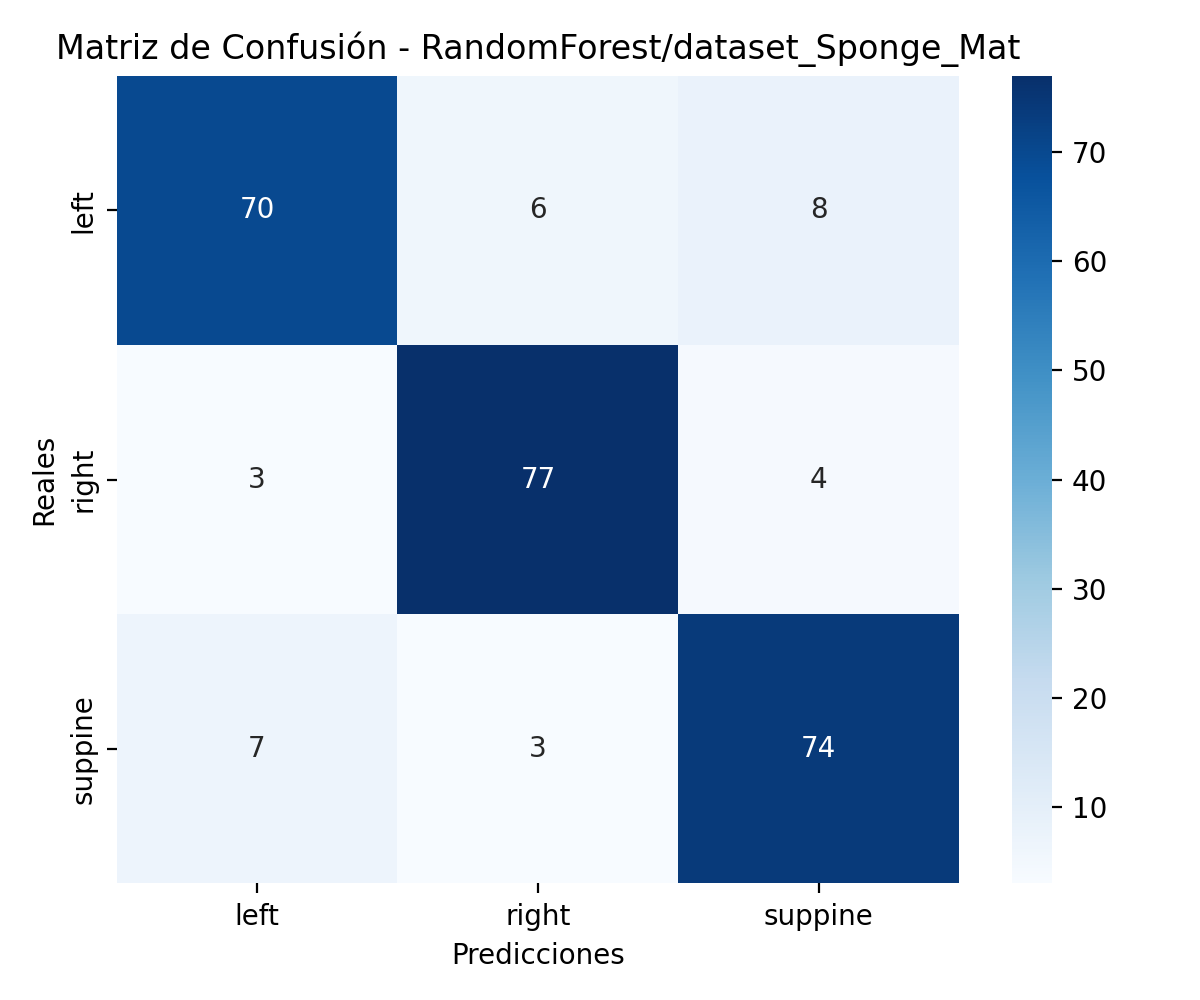
\includegraphics[width=\linewidth]{experimento2/arbol/dataset_Sponge_Mat_confusion_matrix.png}
\caption{1}
\end{subfigure}
\begin{subfigure}{0.3\textwidth}
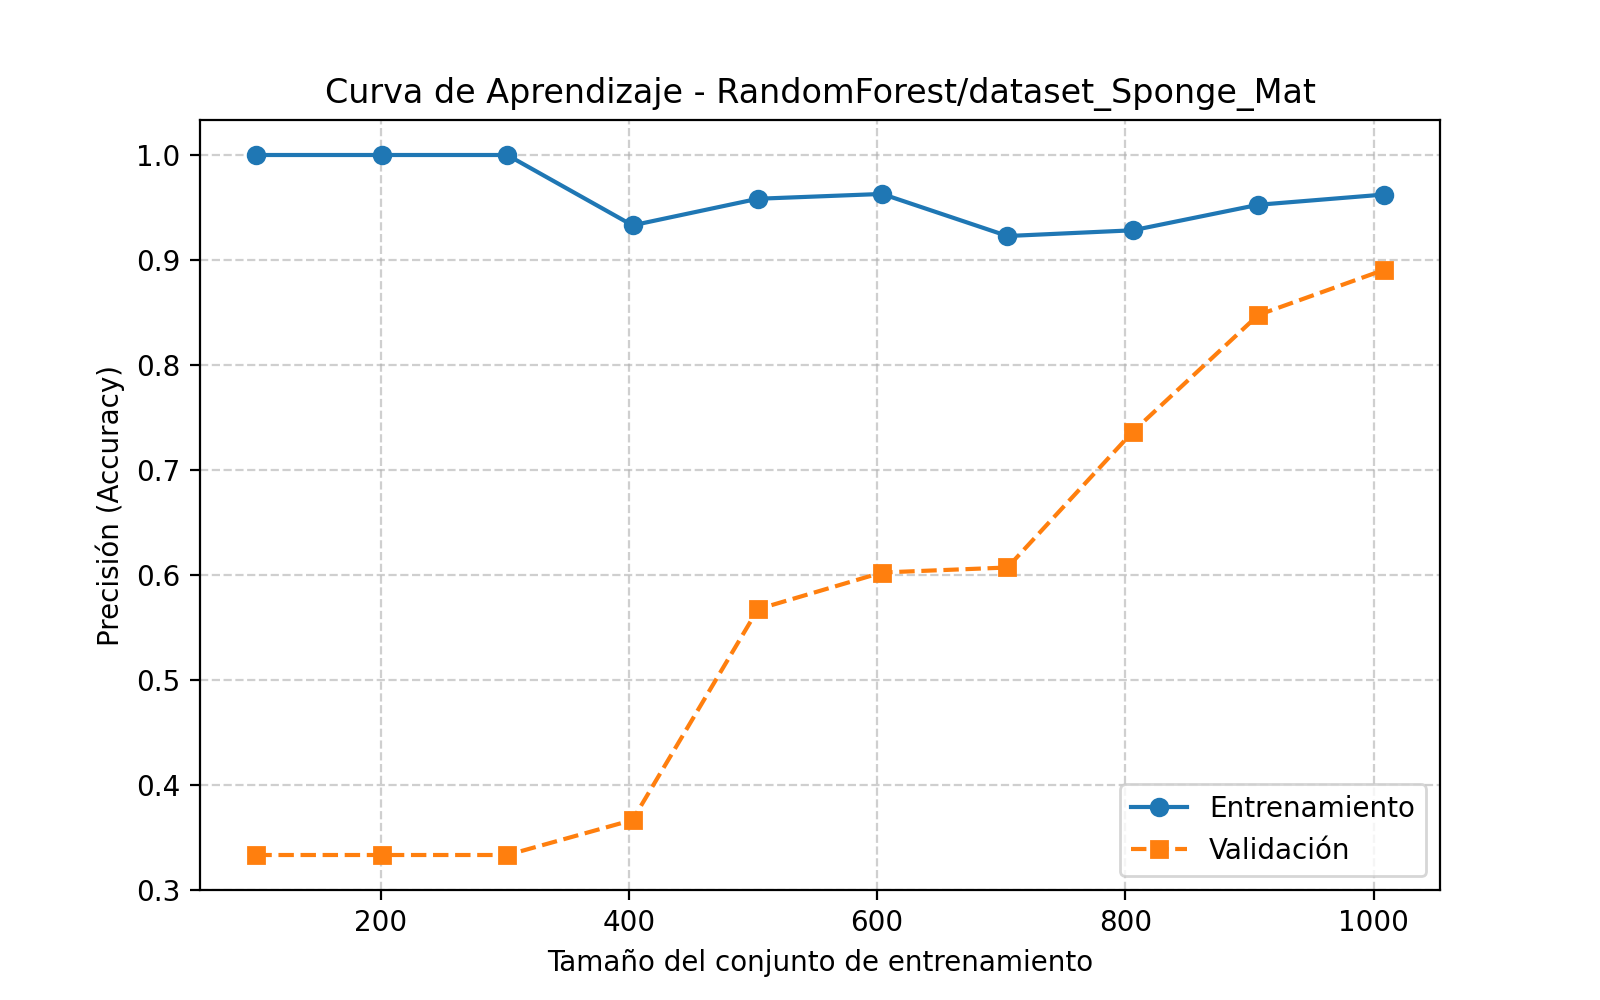
\includegraphics[width=\linewidth]{experimento2/arbol/dataset_Sponge_Mat_learning_curve.png}
\caption{2}
\end{subfigure}
\begin{subfigure}{0.3\textwidth}
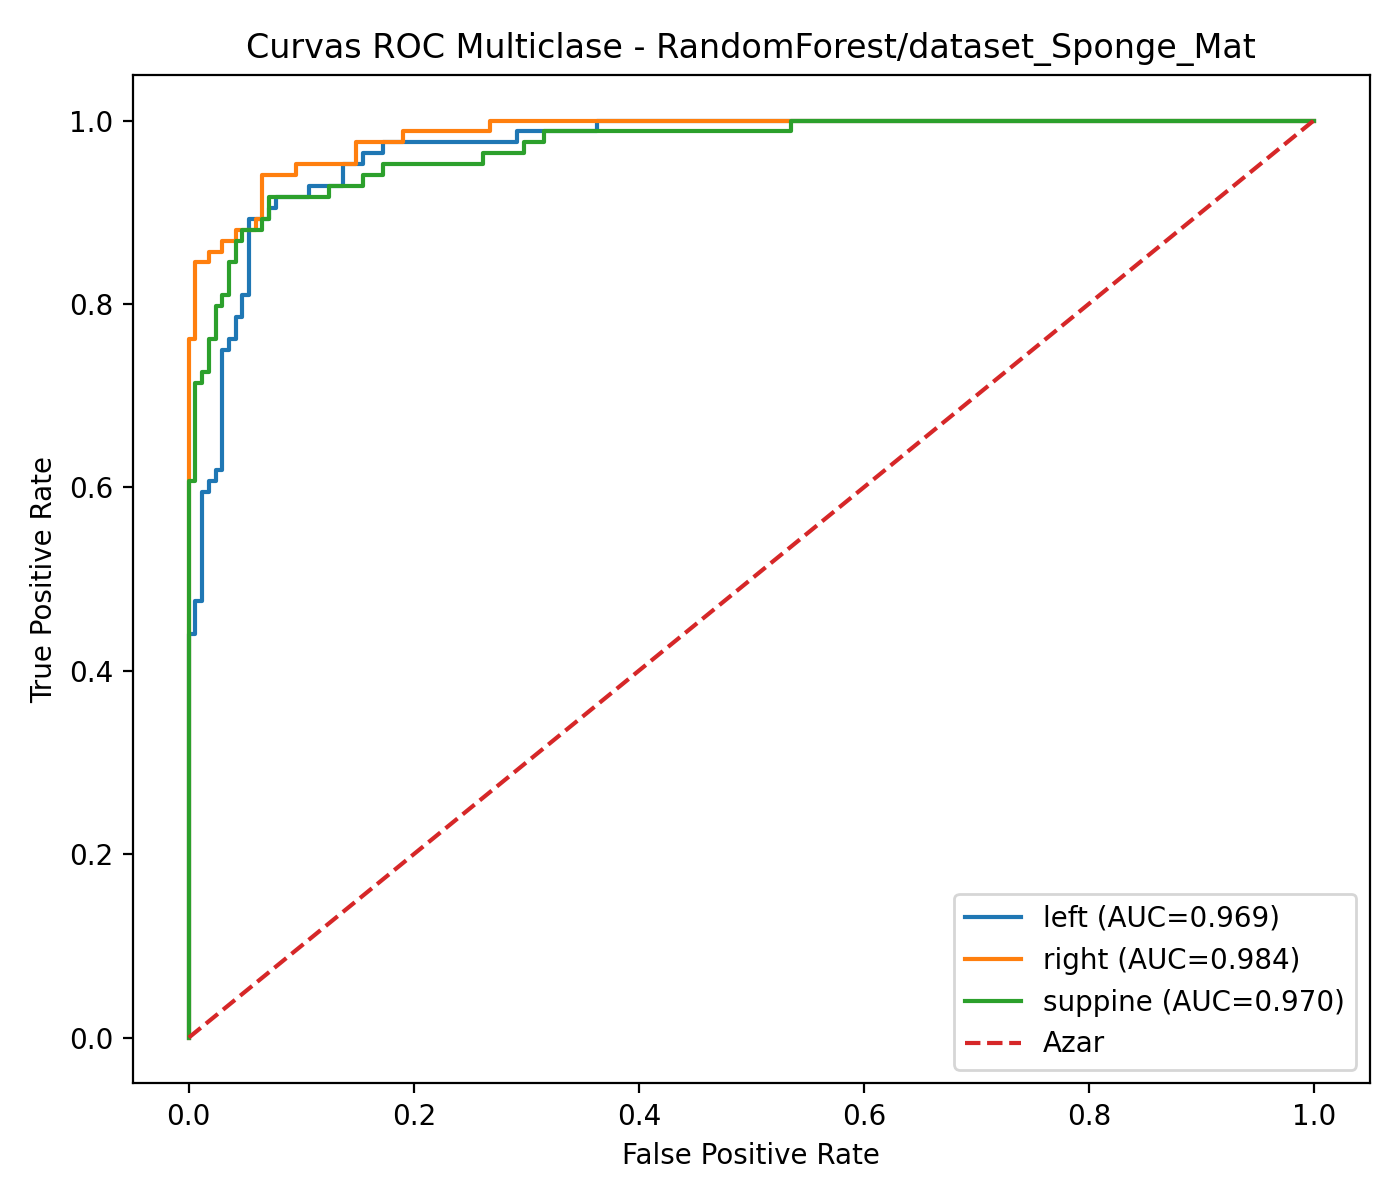
\includegraphics[width=\linewidth]{experimento2/arbol/dataset_Sponge_Mat_multiclass_roc.png}
\caption{3}
\end{subfigure}
\caption{La matriz de confusión, la curva de aprendizaje y la curva ROC para el GradientBoost}
\label{fig:E2GRad}
\end{figure}


\begin{figure}[h!]
\centering

\begin{subfigure}{0.3\textwidth}
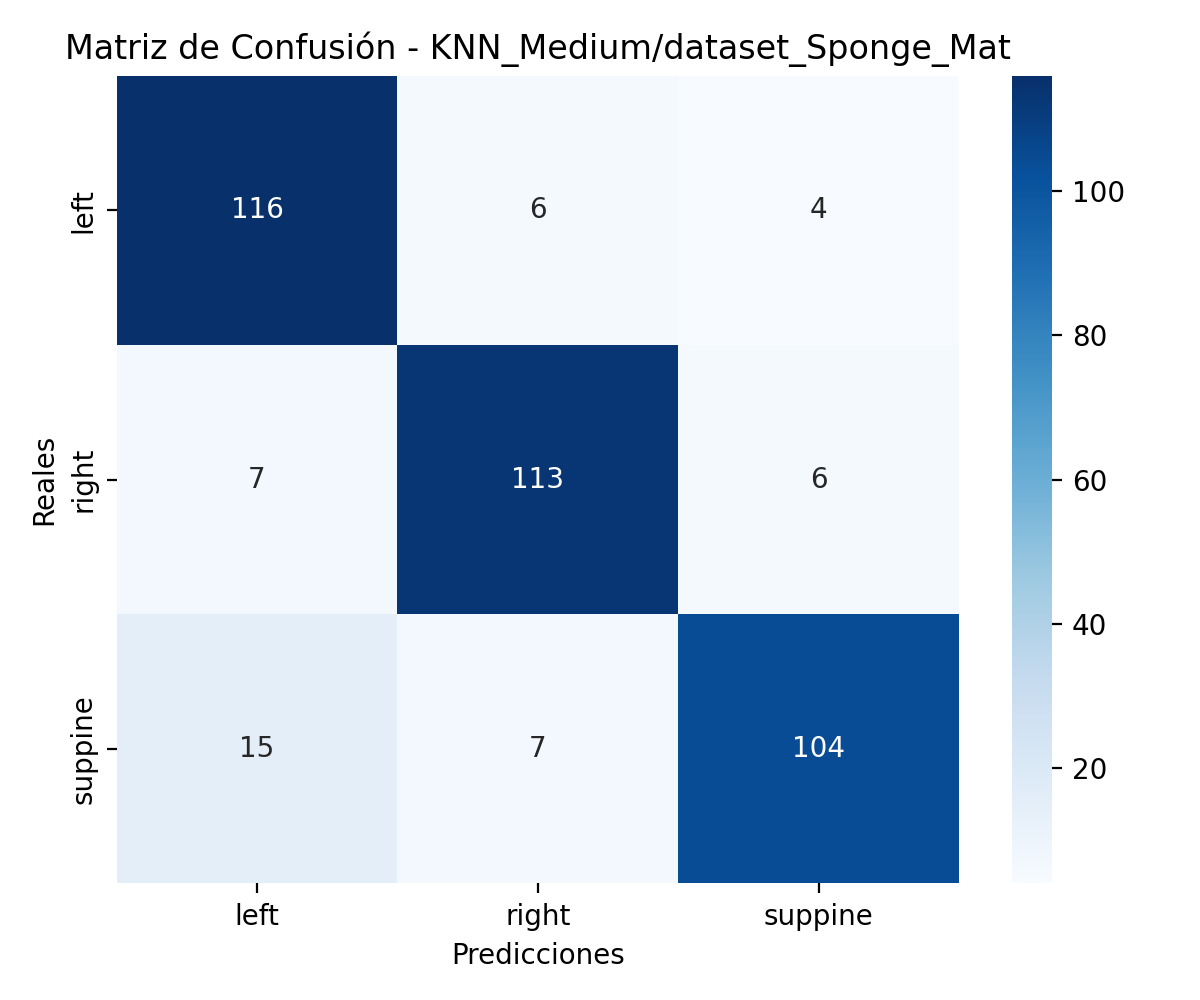
\includegraphics[width=\linewidth]{experimento2/knn/dataset_Sponge_Mat_confusion_matrix.png}
\caption{1}
\end{subfigure}
\begin{subfigure}{0.3\textwidth}
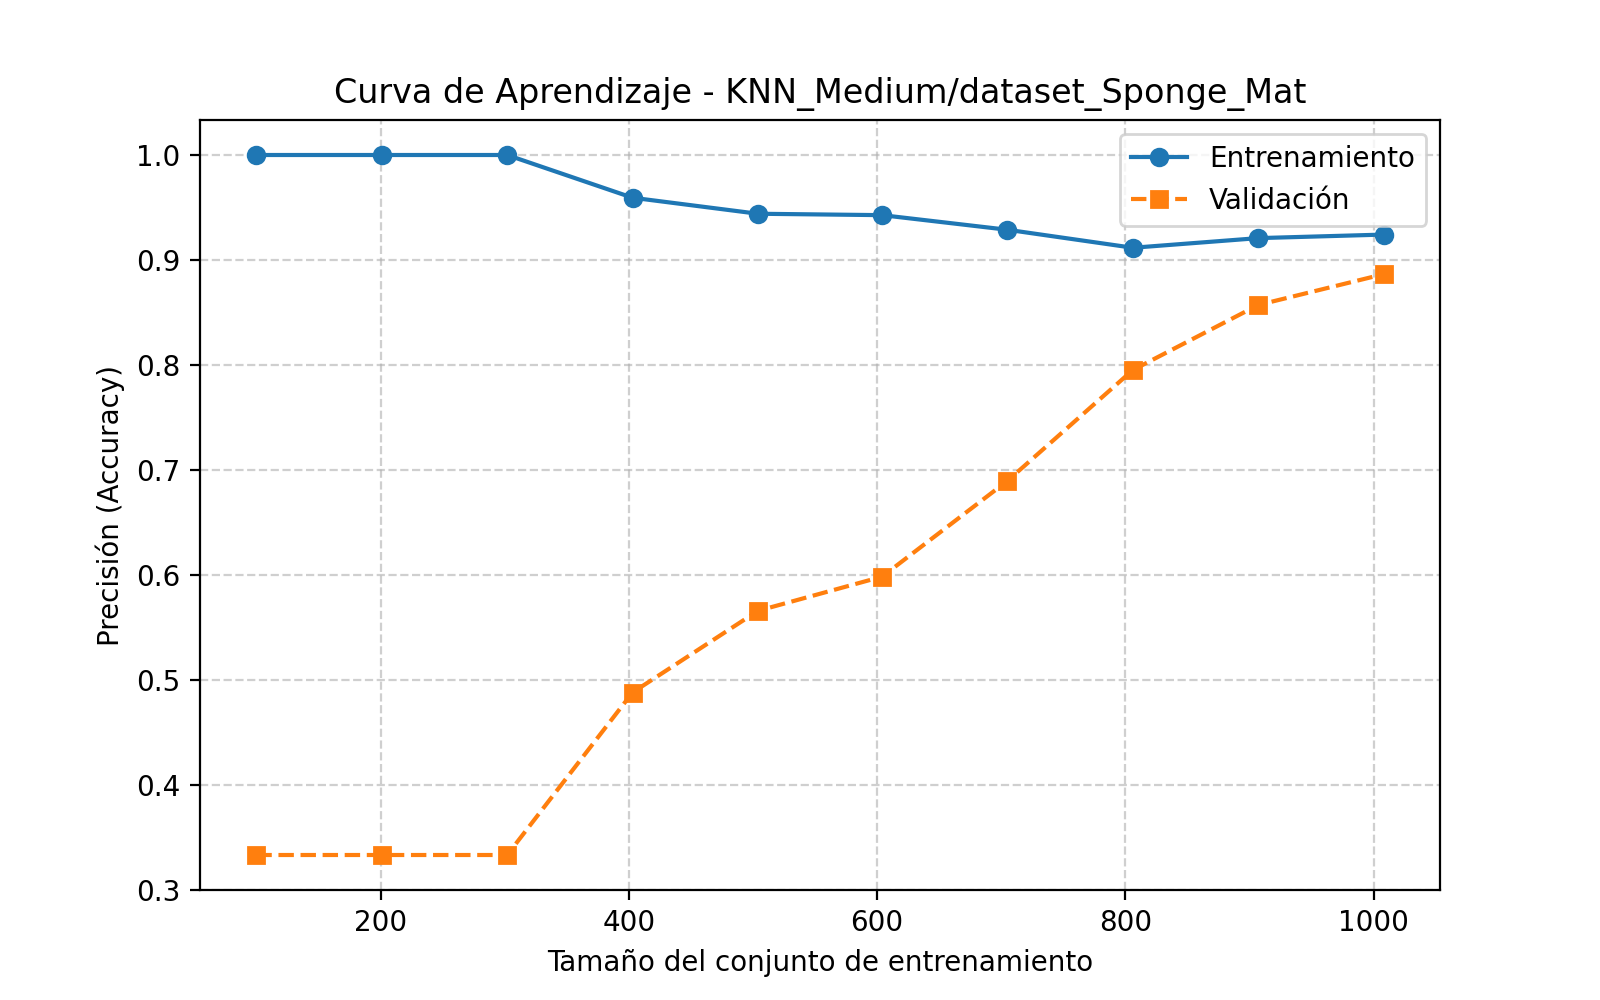
\includegraphics[width=\linewidth]{experimento2/knn/dataset_Sponge_Mat_learning_curve.png}
\caption{2}
\end{subfigure}
\begin{subfigure}{0.3\textwidth}
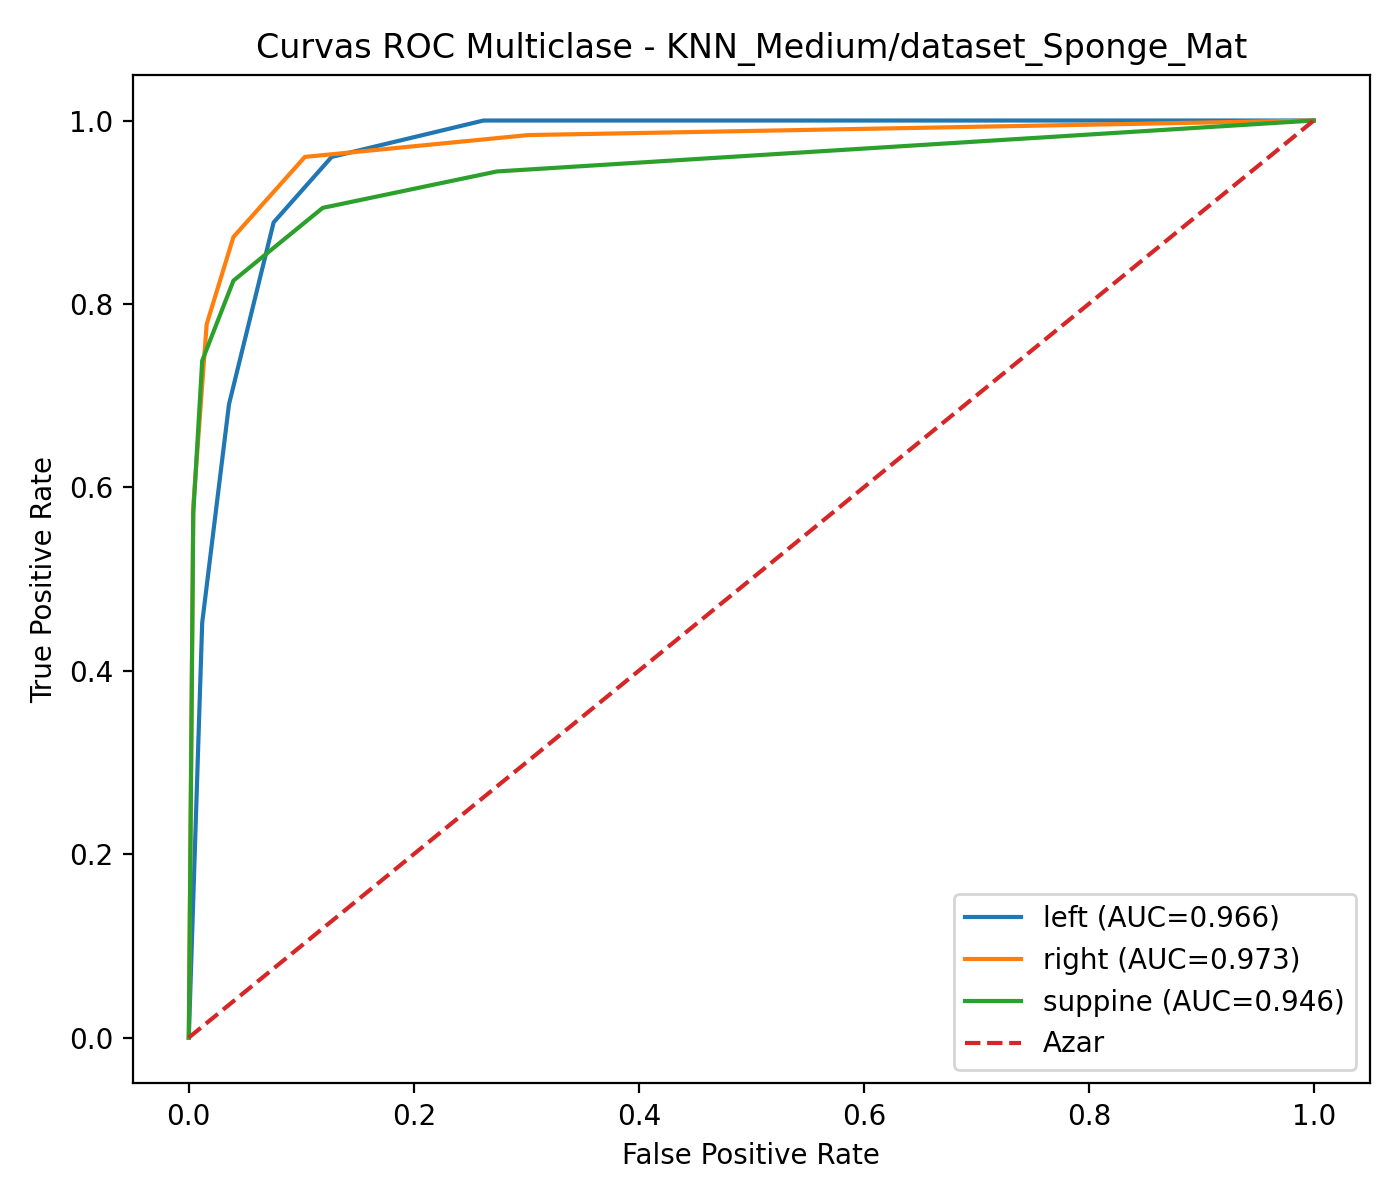
\includegraphics[width=\linewidth]{experimento2/knn/dataset_Sponge_Mat_multiclass_roc.png}
\caption{3}
\end{subfigure}
\caption{La matriz de confusión, la curva de aprendizaje y la curva ROC para el Knn}
\label{fig:E2Knn}
\end{figure}


\begin{figure}[h!]
\centering

\begin{subfigure}{0.3\textwidth}
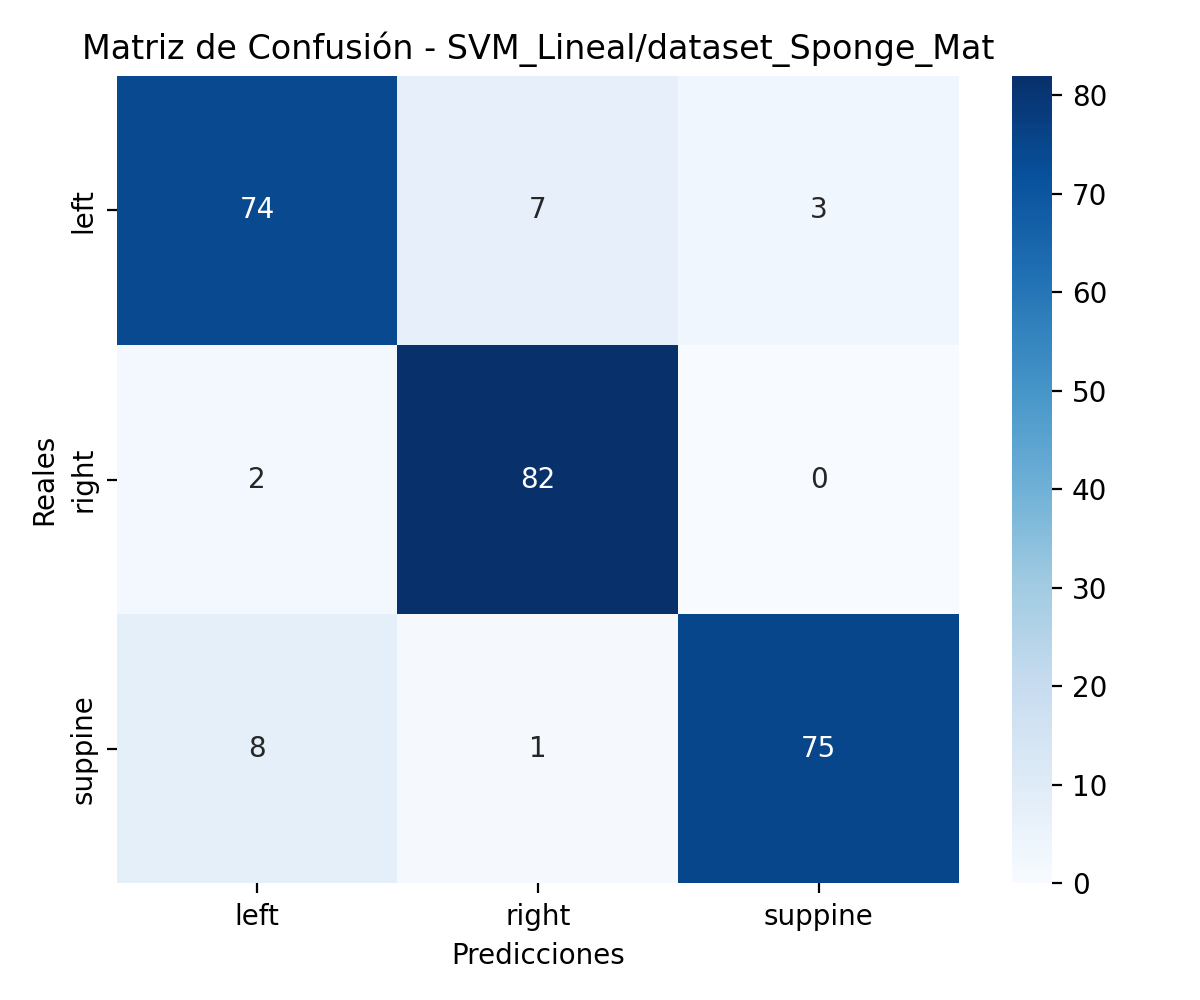
\includegraphics[width=\linewidth]{experimento2/svm/dataset_Sponge_Mat_confusion_matrix.png}
\caption{1}
\end{subfigure}
\begin{subfigure}{0.3\textwidth}
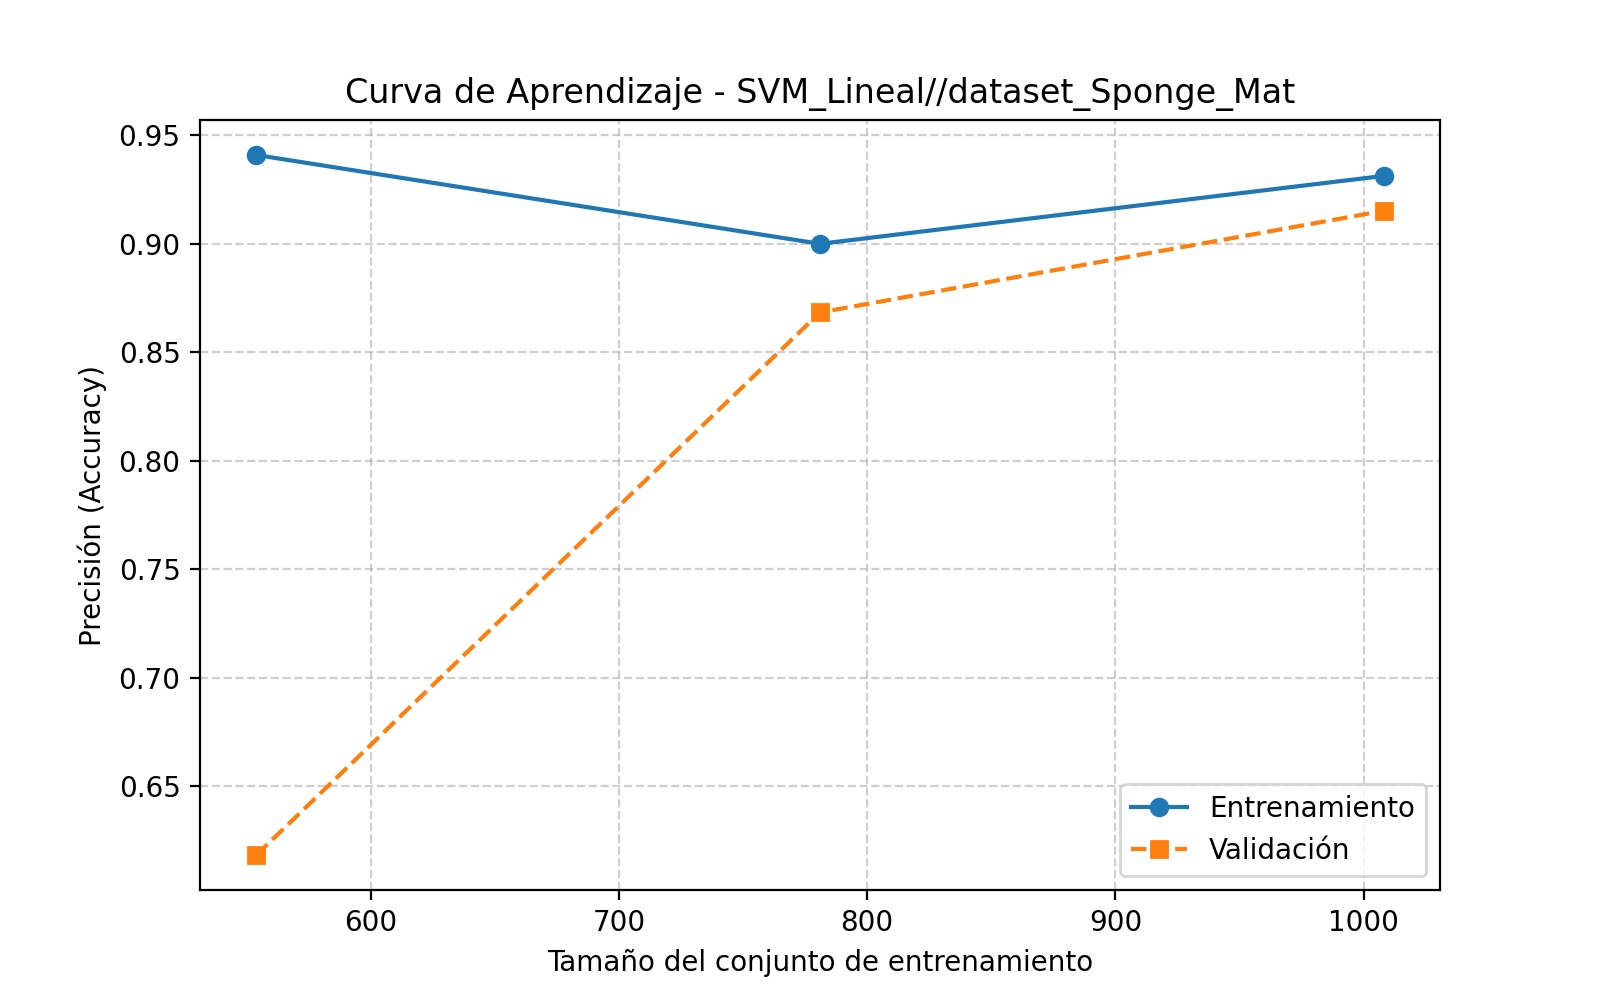
\includegraphics[width=\linewidth]{experimento2/svm/dataset_Sponge_Mat_learning_curve.png}
\caption{2}
\end{subfigure}
\begin{subfigure}{0.3\textwidth}
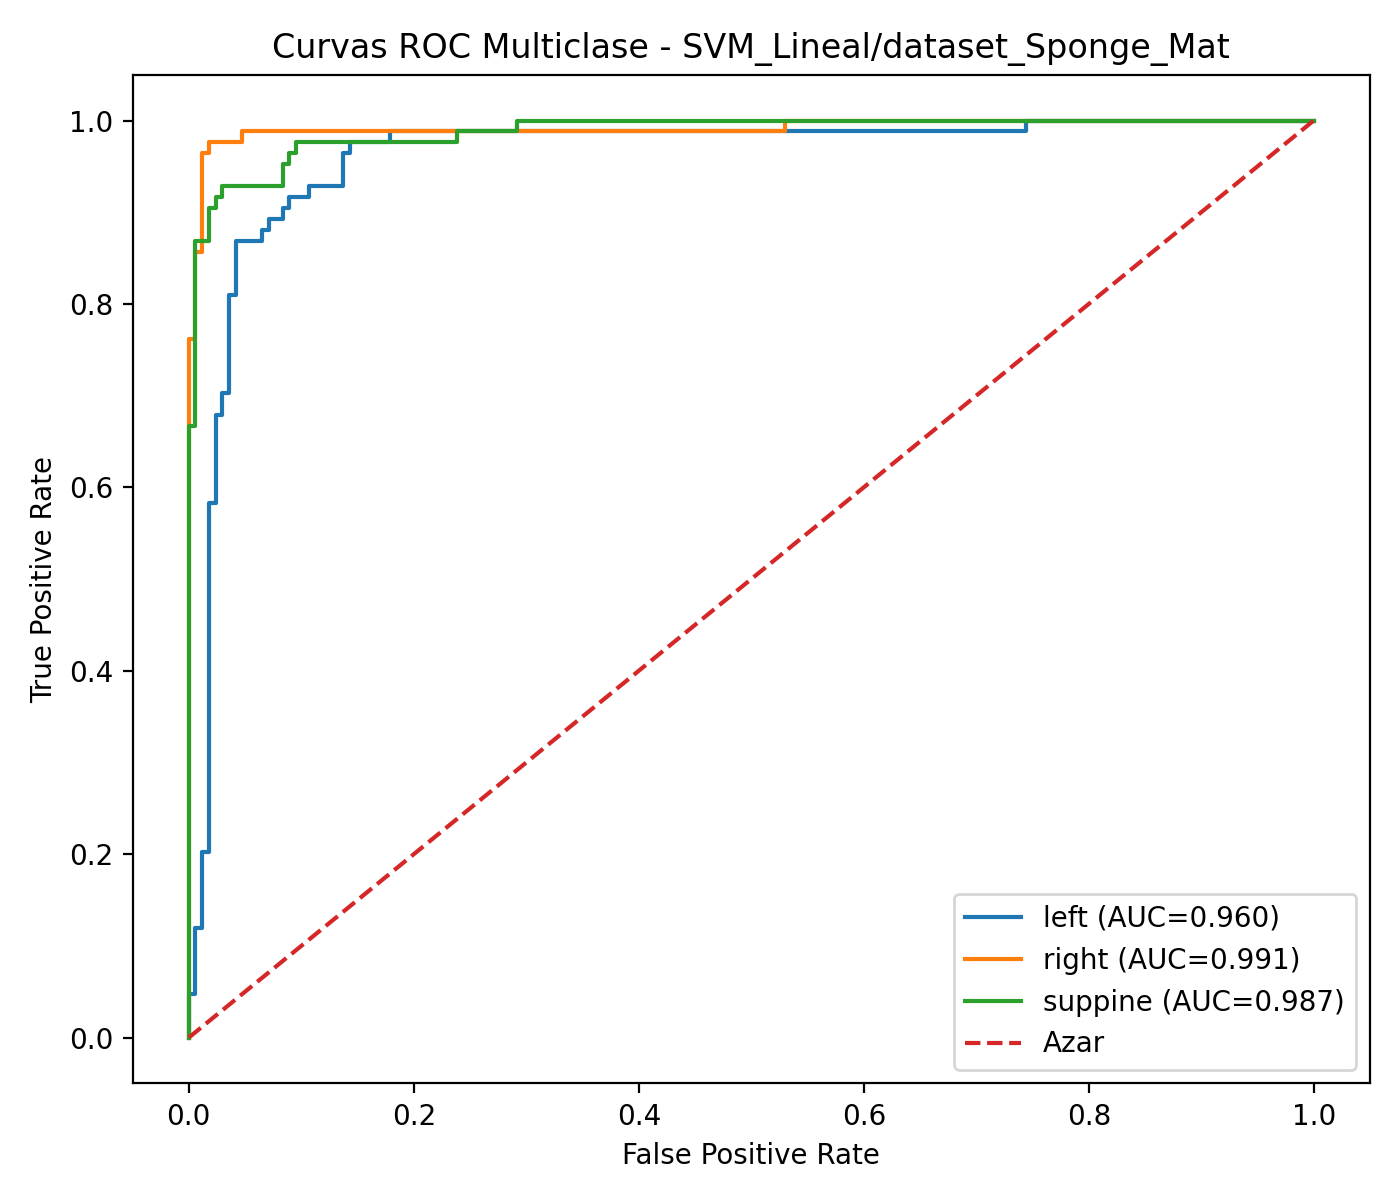
\includegraphics[width=\linewidth]{experimento2/svm/dataset_Sponge_Mat_multiclass_roc.png}
\caption{3}
\end{subfigure}
\caption{La matriz de confusión, la curva de aprendizaje y la curva ROC para el Support Vector Machine}
\label{fig:E2SVM}
\end{figure}


\begin{figure}[h!]
\centering

\begin{subfigure}{0.3\textwidth}
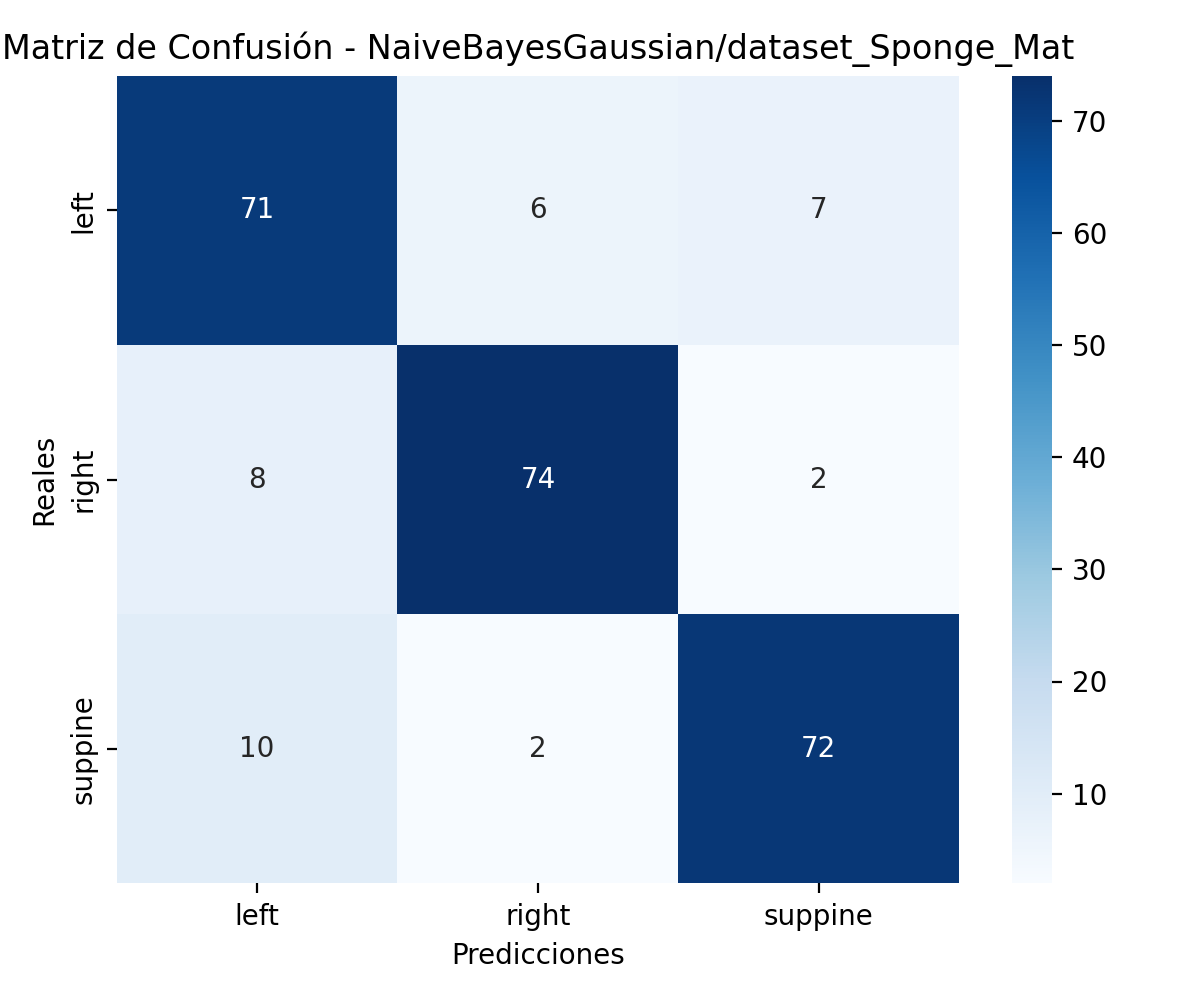
\includegraphics[width=\linewidth]{experimento2/bayesiano/dataset_Sponge_Mat_confusion_matrix.png}
\caption{1}
\end{subfigure}
\begin{subfigure}{0.3\textwidth}
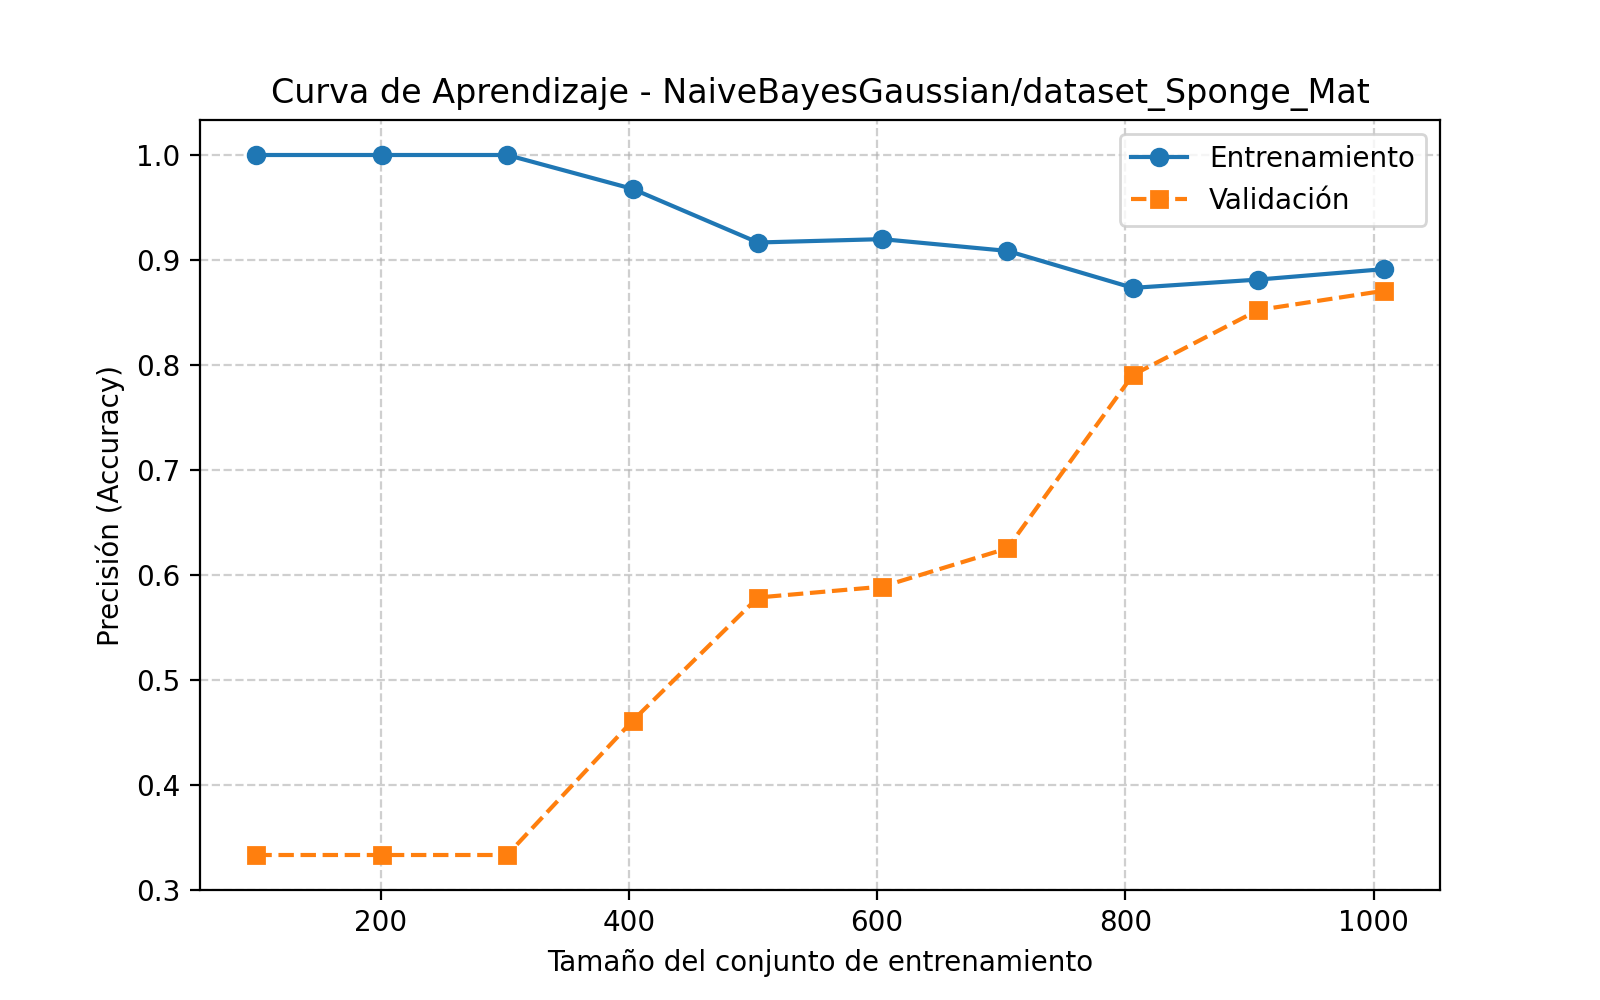
\includegraphics[width=\linewidth]{experimento2/bayesiano/dataset_Sponge_Mat_learning_curve.png}
\caption{2}
\end{subfigure}
\begin{subfigure}{0.3\textwidth}
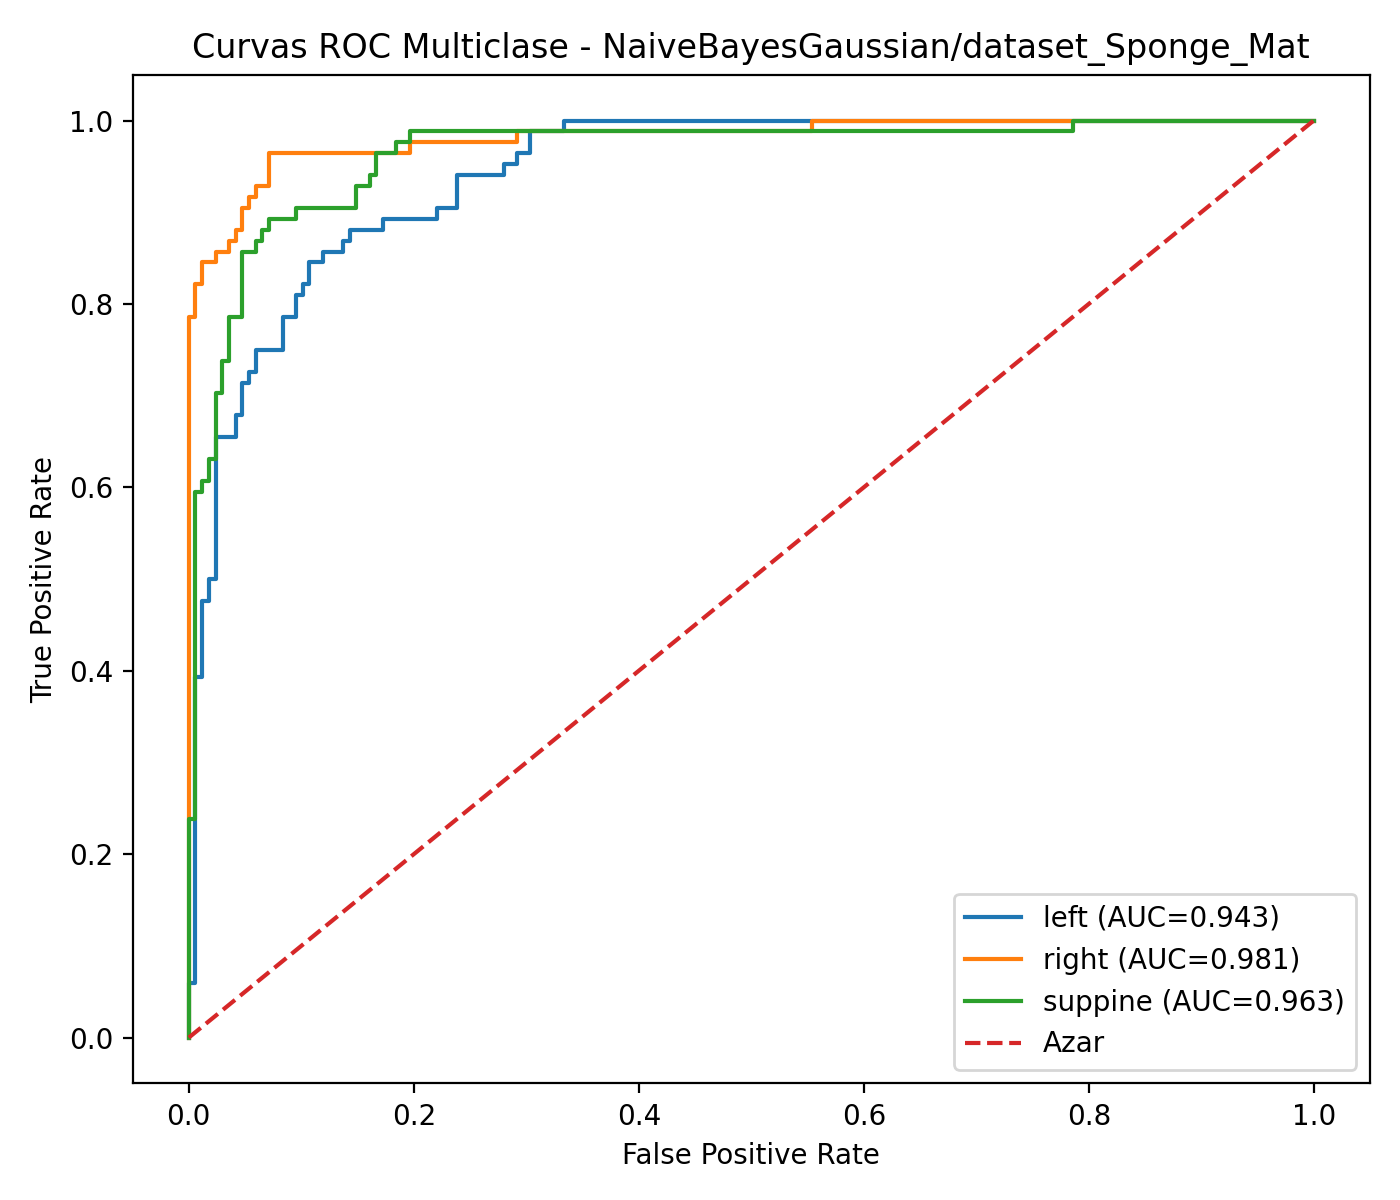
\includegraphics[width=\linewidth]{experimento2/bayesiano/dataset_Sponge_Mat_multiclass_roc.png}
\caption{3}
\end{subfigure}
\caption{La matriz de confusión, la curva de aprendizaje y la curva ROC para el Naive Bayes}
\label{fig:E2Naive}
\end{figure}


\begin{figure}[h!]
\centering

\begin{subfigure}{0.3\textwidth}
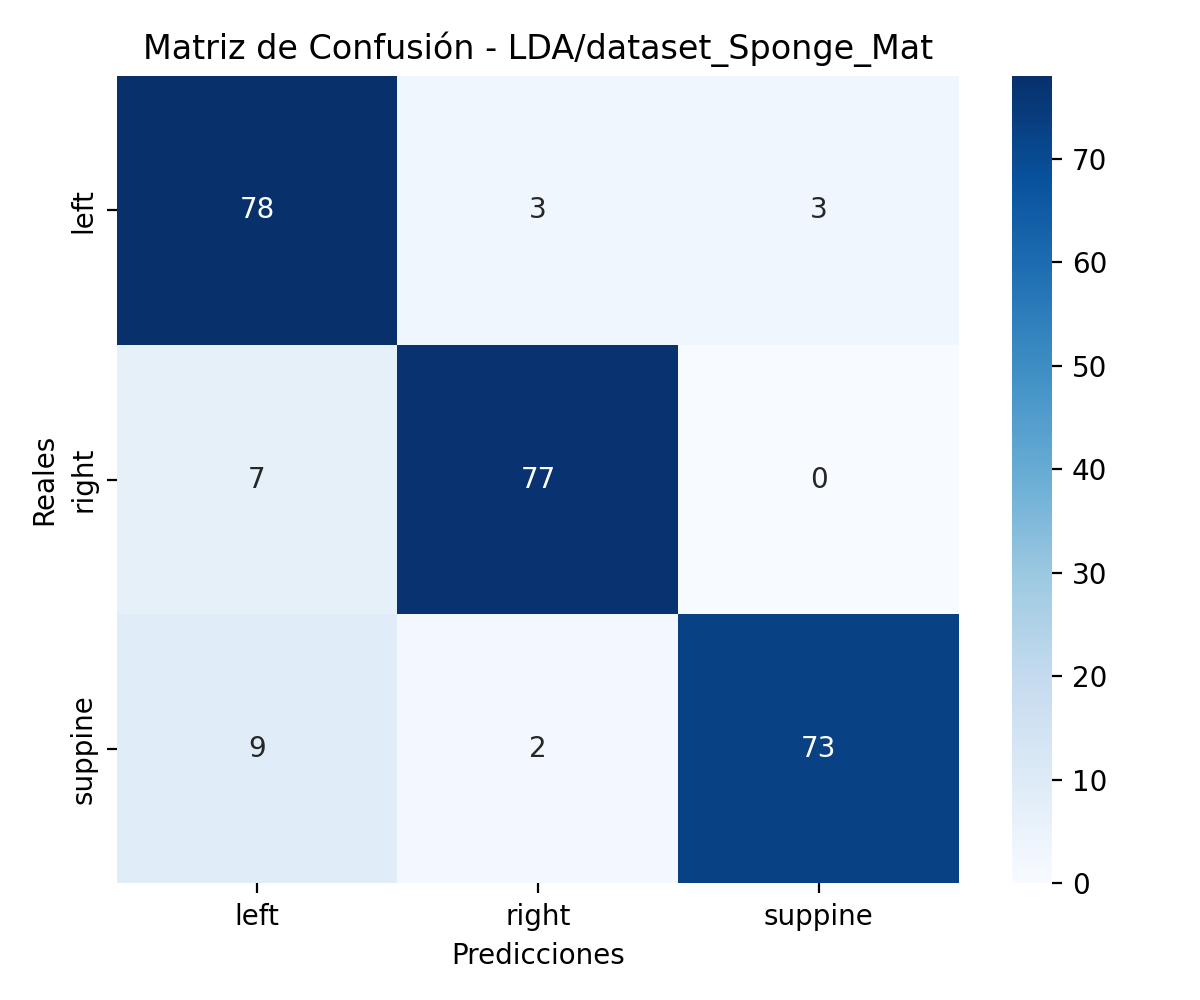
\includegraphics[width=\linewidth]{experimento2/lda/dataset_Sponge_Mat_confusion_matrix.png}
\caption{1}
\end{subfigure}
\begin{subfigure}{0.3\textwidth}
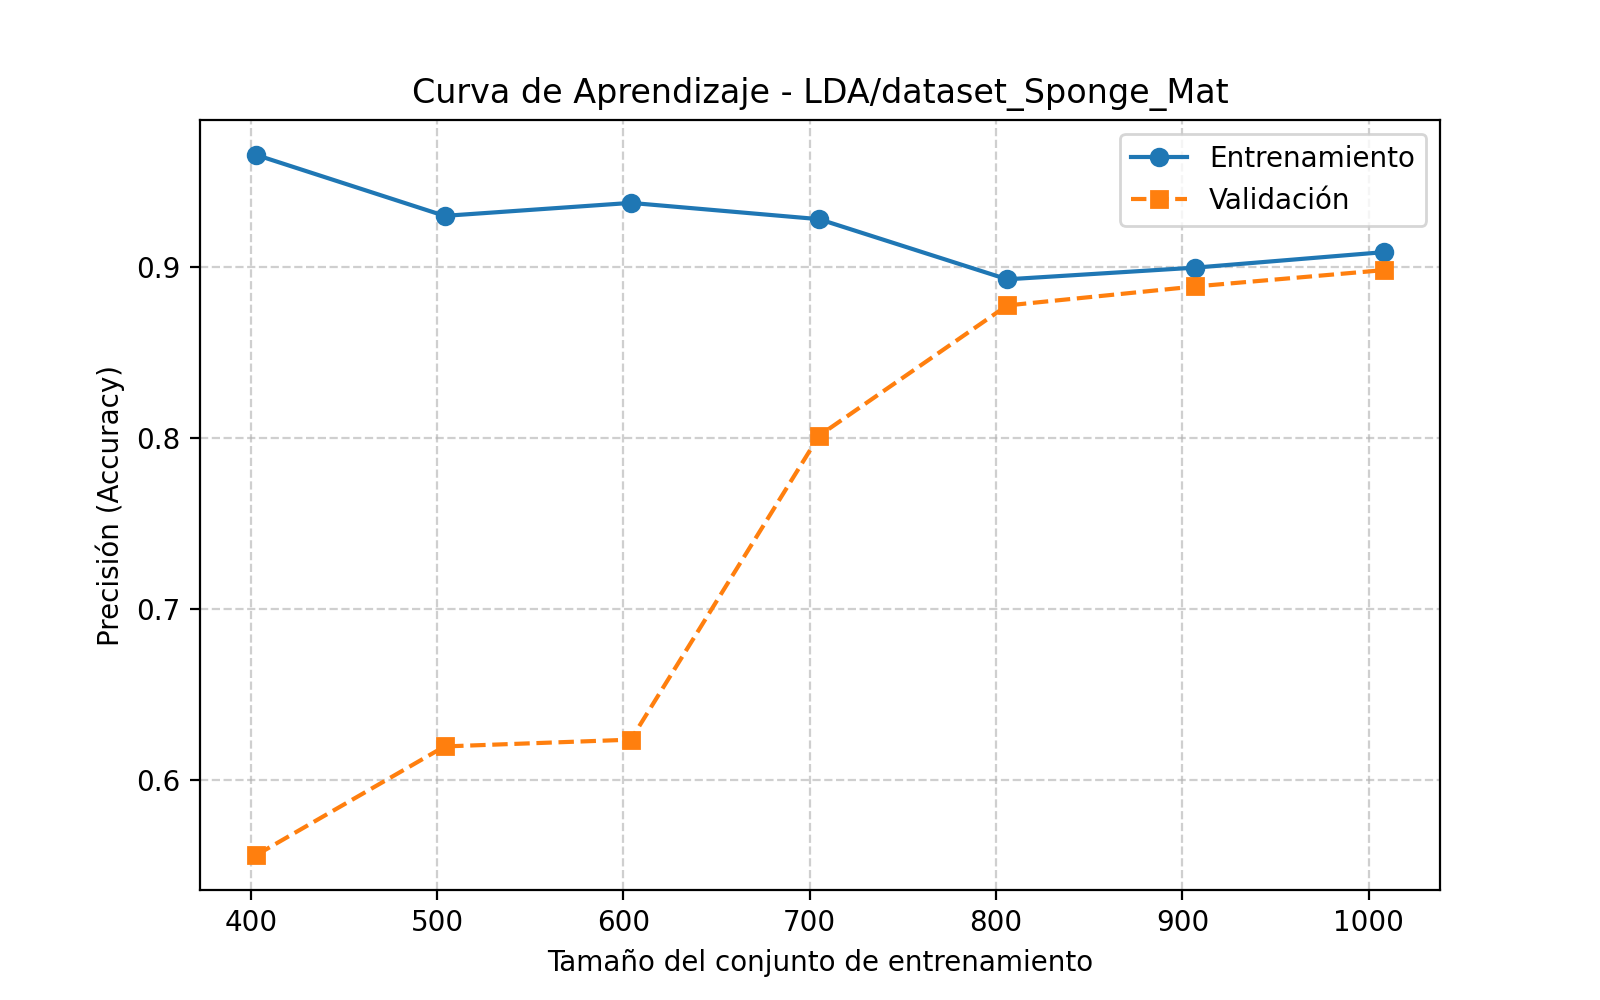
\includegraphics[width=\linewidth]{experimento2/lda/dataset_Sponge_Mat_learning_curve.png}
\caption{2}
\end{subfigure}
\begin{subfigure}{0.3\textwidth}
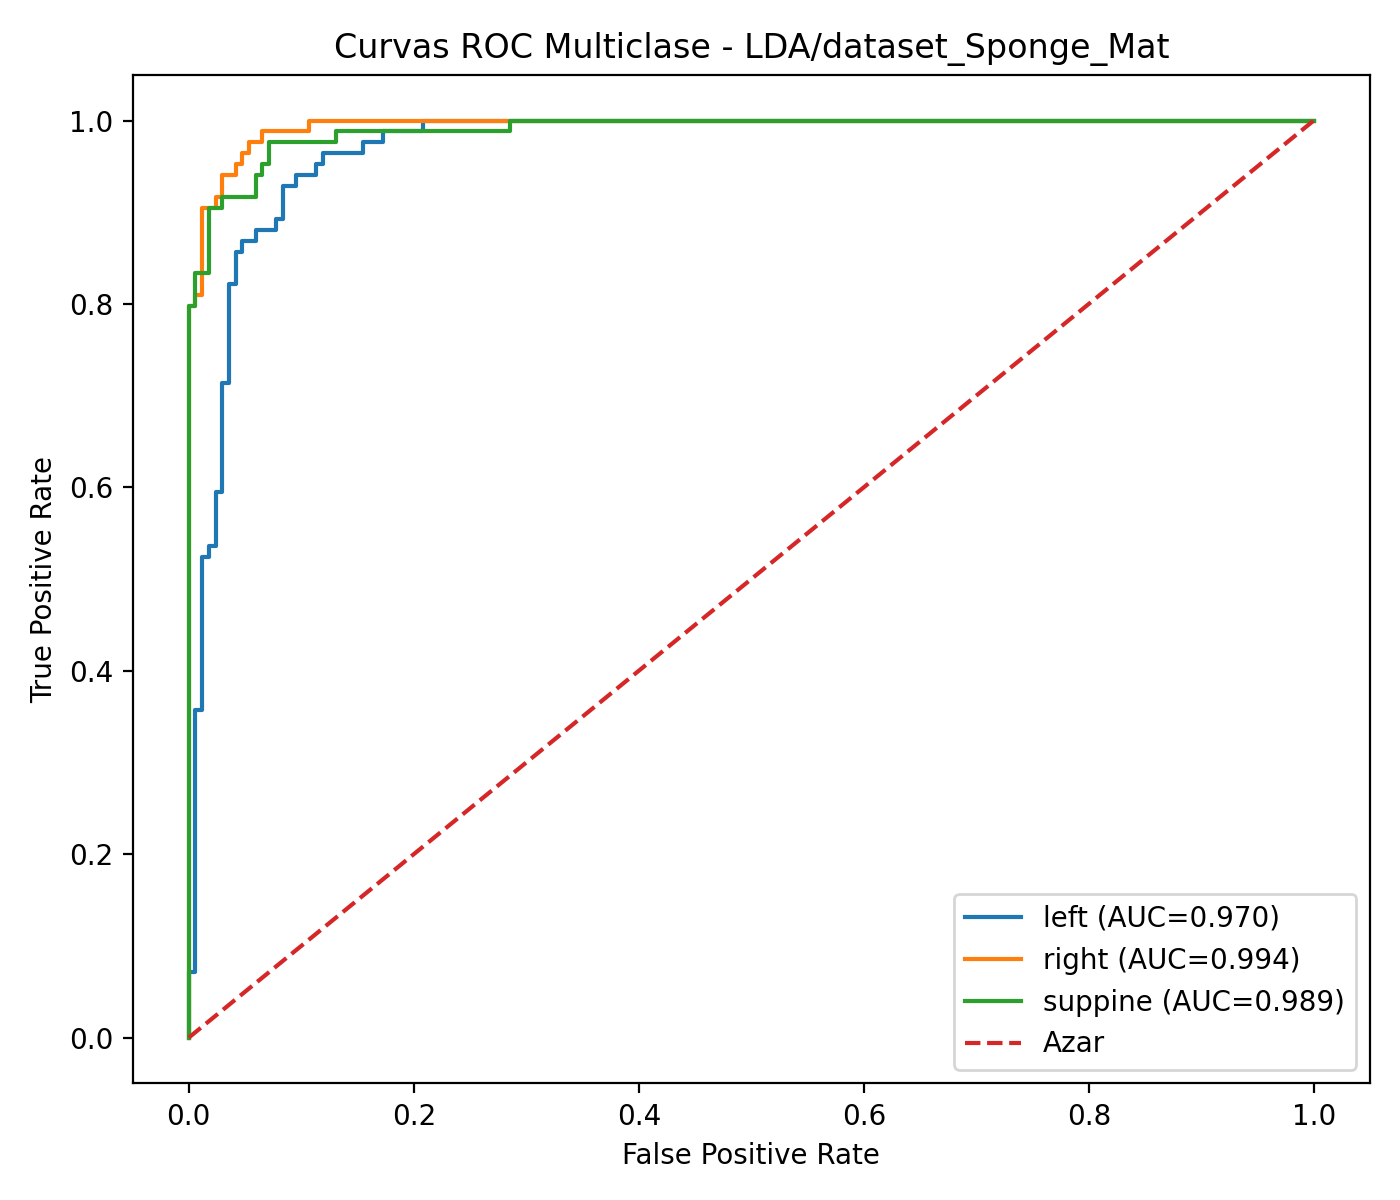
\includegraphics[width=\linewidth]{experimento2/lda/dataset_Sponge_Mat_multiclass_roc.png}
\caption{3}
\end{subfigure}
\caption{La matriz de confusión, la curva de aprendizaje y la curva ROC para el LDA}
\label{fig:E2lda}
\end{figure}
\chapter{Conclusiones}
Los modelos tuvieron un mejor comportamiento cuando se les aplico tanto un escalamiento estándar como un PCA.
Algo que se debe de mencionar, se hizo un primer experimento tomando las características del HoG directamente de la imagen normalizada para agregar los 41 elementos. Resulto en modelos algo pobres, a diferencia de haberlo capturado de otro HoG con 9 bins. Además, el escalamiento estándar y la reducción de dimensionalidad ayudó a los modelos a mejorar sus curvas, sobre todo aquellos modelos que son de árboles.
Knn no presentó mejoras significativas con el uso de PCA, a diferencia de otros modelos. Este problema muestra que se necesita bastante información para que los modelos puedan ser de mejor calidad. Ya que en un principio, tienden al sobre ajuste
\bibliographystyle{ieeetr}
\bibliography{reference}

\end{document} 